\documentclass[aspectratio=169,11pt]{beamer}

\newcommand{\currentpart}{5}
% ============================================================================
% Quantitative Research -- shared preamble for all five slide decks
%
% Every deck starts with
%     \documentclass[aspectratio=169,11pt]{beamer}
%     % ============================================================================
% Quantitative Research -- shared preamble for all five slide decks
%
% Every deck starts with
%     \documentclass[aspectratio=169,11pt]{beamer}
%     % ============================================================================
% Quantitative Research -- shared preamble for all five slide decks
%
% Every deck starts with
%     \documentclass[aspectratio=169,11pt]{beamer}
%     \input{../common/preamble.tex}
%     \newcommand{\currentpart}{<k>}
% so that layout, colours, boxes and code listings are identical everywhere.
% ============================================================================

% ======================== Packages ========================
\usepackage[utf8]{inputenc}
\usepackage[T1]{fontenc}
\usepackage[english]{babel}
\usepackage{graphicx}
\usepackage{booktabs}
\usepackage{amsmath,amssymb,amsfonts}
\usepackage{mathtools}
\usepackage{xcolor}
\usepackage{colortbl}
\usepackage{array}
\usepackage{multicol}
\usepackage{verbatim}          % provides the comment environment
\usepackage{tikz}
\usepackage{pgfplots}
\pgfplotsset{compat=1.18}
\usetikzlibrary{arrows.meta,positioning,fit,backgrounds,shapes.geometric,calc,decorations.pathreplacing}
\usepackage{listings}
\usepackage{hyperref}
\usepackage{pgfpages}          % notes on a second screen (only if enabled)

% ======================== Speaker notes (talk-tracks) ========================
% The decks compile WITHOUT notes by default. To get a version with the
% talk-tracks, uncomment exactly ONE of the lines below and recompile:
% \setbeameroption{show notes}                          % notes as separate pages
% \setbeameroption{show notes on second screen=right}   % slides left, notes right

% ======================== Math fonts ========================
% Beamer typesets text in sans serif; make \mathrm and \mathbf match it
% (otherwise SE, TP, RSS print in serif and \mathbf falls back to non-bold).
\renewcommand{\bfdefault}{bx}   % CM sans has bold extended (bx) only
\DeclareMathAlphabet{\mathrm}{T1}{cmss}{m}{n}
\DeclareMathAlphabet{\mathbf}{T1}{cmss}{bx}{n}
\SetMathAlphabet{\mathrm}{bold}{T1}{cmss}{bx}{n}
\SetMathAlphabet{\mathbf}{bold}{T1}{cmss}{bx}{n}
\SetSymbolFont{operators}{bold}{OT1}{cmss}{bx}{n}
% Beamer re-declares \mathrm at \begin{document}; re-apply the sans-serif version
\AtBeginDocument{\SetMathAlphabet{\mathrm}{normal}{T1}{cmss}{m}{n}%
                 \SetMathAlphabet{\mathrm}{bold}{T1}{cmss}{bx}{n}}

% ======================== Colour palette (matched to plots / Madrid) ========
\definecolor{hsbiblau}{HTML}{3333B2}
\definecolor{hsbiblaudunkel}{HTML}{1C1C6E}
\definecolor{hsbiorange}{HTML}{E69F00}
\definecolor{hsbigrau}{HTML}{9A9A9A}
\definecolor{hsbirot}{HTML}{C0392B}
\definecolor{hsbigruen}{HTML}{2E8B57}
\definecolor{hsbiviolett}{HTML}{8C3CA0}   % 4th comparison colour (e.g. candidate lines)

% ======================== Theme ========================
\usetheme{Madrid}
\usecolortheme{default}
\setbeamertemplate{navigation symbols}{}
\setbeamertemplate{blocks}[rounded][shadow=false]
\setbeamerfont{section in head/foot}{size=\tiny}

% Horizontal section navigation bar in the headline
\setbeamertemplate{headline}{%
  \leavevmode%
  \hbox{%
    \begin{beamercolorbox}[wd=\paperwidth,ht=2.5ex,dp=1.125ex]{section in head/foot}%
      \scriptsize\insertsectionnavigationhorizontal{\paperwidth}{}{\hskip0pt plus1filll}%
    \end{beamercolorbox}%
  }%
}

% Footline: lecture part, current section (if any) and slide number
\newcommand{\footsection}{%
  \setbox0=\hbox{\insertsection}%
  \ifdim\wd0>0pt\ \textbar\ \insertsection\fi}
\setbeamertemplate{footline}{%
  \leavevmode%
  \hbox{%
  \begin{beamercolorbox}[wd=\paperwidth,ht=2.5ex,dp=1.125ex]{author in head/foot}%
    \hspace*{2em}Part~\currentpart\footsection\hfill\insertframenumber{}/\inserttotalframenumber\hspace*{2em}%
  \end{beamercolorbox}%
  }%
}

% Automatic section overview slide. Decks with many sections define
%   \newcommand{\overviewleft}{1-4}\newcommand{\overviewright}{5-8}
% before \begin{document} to get a two-column overview.
\newcommand{\overviewtoc}[1]{%
  \tableofcontents[currentsection,sectionstyle=show/shaded,
                   subsectionstyle=show/show/hide,sections={#1}]}
\newcommand{\sectionoverview}{%
  \ifdefined\overviewleft
    \begin{columns}[T]
      \column{0.49\textwidth}\overviewtoc{\overviewleft}
      \column{0.49\textwidth}\overviewtoc{\overviewright}
    \end{columns}%
  \else
    \tableofcontents[currentsection,sectionstyle=show/shaded,
                     subsectionstyle=show/show/hide]%
  \fi}
\AtBeginSection[]{%
  \begin{frame}{Overview}
    \scriptsize
    \sectionoverview
  \end{frame}%
}

% ======================== Python listing style ========================
\lstdefinestyle{Pystyle}{
  language=Python,
  basicstyle=\ttfamily\footnotesize,
  keywordstyle=\color{hsbiblau},
  commentstyle=\color{hsbigrau}\itshape,
  stringstyle=\color{teal},
  showstringspaces=false,
  literate={~}{{$\sim$}}1
           {–}{{--}}1 {—}{{---}}1 {ä}{{\"a}}1 {ö}{{\"o}}1 {ü}{{\"u}}1
           {Ä}{{\"A}}1 {Ö}{{\"O}}1 {Ü}{{\"U}}1 {ß}{{\ss}}1 {é}{{\'e}}1,
  upquote=true,
  columns=fixed, basewidth=0.5em
}
% Plain style for printed Python output (fixed columns keep tables aligned)
\lstdefinestyle{Pyout}{
  language={},
  basicstyle=\ttfamily\scriptsize,
  keywordstyle={}, commentstyle={}, stringstyle={},
  columns=fixed, keepspaces=true, basewidth=0.52em,
  showstringspaces=false,
  upquote=true,
  literate={~}{{$\sim$}}1 {–}{{--}}1 {—}{{---}}1 {‘}{{`}}1 {’}{{'}}1,
}
\lstset{style=Pystyle}

% ======================== Custom commands / styles ========================
\newcommand{\kernaussage}[1]{\begin{alertblock}{Key takeaway}#1\end{alertblock}}
\newcommand{\inworten}[1]{{\small\textbf{\textcolor{hsbiblaudunkel}{In words:}}~#1}}
\newcommand{\guidingquestion}[1]{\begin{exampleblock}{Guiding question}#1\end{exampleblock}}
\newcommand{\appendixnote}[1]{\par\vfill\vspace{-1.6ex}\hfill{\scriptsize\itshape\textcolor{hsbiblau}{$\rightarrow$ Appendix: #1}}\par\vspace{-1ex}}
\newcommand{\sourcenote}[1]{\vfill\hfill{\tiny\itshape\color{gray}Source: #1}\par}

% Companion notebooks (Jupyter / Google Colab). Every deck defines
%     \newcommand{\notebookpath}{Part_k_<Topic>/Part_k_<Topic>.ipynb}
% \trynotebook{<notebook section>} prints a small clickable pointer at the
% bottom right of a frame that opens the deck's notebook in Google Colab
% (the same notebook lies next to the .tex file for local Jupyter use).
\newcommand{\colaburl}{https://colab.research.google.com/github/ChrisW09/Quantitative-Research-Methods/blob/main/}
\newcommand{\trynotebook}[1]{\par\vfill\vspace{-1.6ex}\hfill{\scriptsize\href{\colaburl\notebookpath}{\textcolor{hsbiorange!85!black}{$\blacktriangleright$\ \textbf{Try it yourself:} notebook, #1 \ -- open in Colab}}}\par\vspace{-1ex}}

% Reusable TikZ styles for concept diagrams
\tikzset{
  flowbox/.style={rounded corners, draw=hsbiblaudunkel, very thick,
                  fill=hsbiblau!10, align=center, inner sep=5pt, minimum height=8mm},
  flowboxo/.style={rounded corners, draw=hsbiorange!85!black, very thick,
                   fill=hsbiorange!18, align=center, inner sep=5pt, minimum height=8mm},
  flowboxg/.style={rounded corners, draw=hsbigrau!90!black, very thick,
                   fill=hsbigrau!15, align=center, inner sep=5pt, minimum height=8mm},
  flowarr/.style={-{Latex[length=2.6mm,width=2mm]}, line width=1pt, draw=hsbiblaudunkel},
}

% ======================== Course overview (same slide in every deck) ========
% \courseoverview highlights the part given by \currentpart.
\newcommand{\cpart}[2]{%
  \ifnum\currentpart=#1\relax
    \textcolor{hsbiblau}{\textbf{#2}}%
  \else
    #2%
  \fi}
\newcommand{\courseoverview}{%
\begin{frame}{The lecture at a glance}
  \begin{center}
    \small\renewcommand{\arraystretch}{1.15}
    \begin{tabular}{@{}l l >{\raggedright\arraybackslash}p{9.2cm}@{}}
      \toprule
      & \textbf{Part} & \textbf{Content} \\
      \midrule
      \ifnum\currentpart=1 $\blacktriangleright$\fi & \cpart{1}{1 -- Descriptive Statistics}
        & \cpart{1}{Basic concepts, levels of measurement, frequencies, measures of central tendency and dispersion} \\
      \ifnum\currentpart=2 $\blacktriangleright$\fi & \cpart{2}{2 -- Graphical Representations}
        & \cpart{2}{Empirical CDF, histogram, boxplot} \\
      \ifnum\currentpart=3 $\blacktriangleright$\fi & \cpart{3}{3 -- Statistical Inference}
        & \cpart{3}{Normal distribution and CLT, confidence intervals, sample size, hypothesis tests, $p$-values, one-sided tests, types of error} \\
      \ifnum\currentpart=4 $\blacktriangleright$\fi & \cpart{4}{4 -- Regression}
        & \cpart{4}{Correlation, least squares, goodness of fit, inference for regression, multiple regression (appendix: residual analysis)} \\
      \ifnum\currentpart=5 $\blacktriangleright$\fi & \cpart{5}{5 -- Classification}
        & \cpart{5}{Conditional probability, logistic regression, classification rules, confusion matrix, base rates, ROC/AUC, Bayes classifiers} \\
      \bottomrule
    \end{tabular}
  \end{center}
  \begin{center}
    \footnotesize All analyses are carried out in \textbf{Python} (NumPy,
    pandas, SciPy, statsmodels, matplotlib); every deck comes with a Python
    script that reproduces its numbers and a Jupyter notebook with all
    examples and exercises -- also in Google Colab.
  \end{center}
\end{frame}}

% ======================== Title information (shared) ========================
\title{Quantitative Research}
\author{Prof.\ Dr.\ Christoph Weisser}
\institute{}
\date{}   % must stay explicitly empty -- otherwise Beamer prints today's date

\graphicspath{{images/}}

%     \newcommand{\currentpart}{<k>}
% so that layout, colours, boxes and code listings are identical everywhere.
% ============================================================================

% ======================== Packages ========================
\usepackage[utf8]{inputenc}
\usepackage[T1]{fontenc}
\usepackage[english]{babel}
\usepackage{graphicx}
\usepackage{booktabs}
\usepackage{amsmath,amssymb,amsfonts}
\usepackage{mathtools}
\usepackage{xcolor}
\usepackage{colortbl}
\usepackage{array}
\usepackage{multicol}
\usepackage{verbatim}          % provides the comment environment
\usepackage{tikz}
\usepackage{pgfplots}
\pgfplotsset{compat=1.18}
\usetikzlibrary{arrows.meta,positioning,fit,backgrounds,shapes.geometric,calc,decorations.pathreplacing}
\usepackage{listings}
\usepackage{hyperref}
\usepackage{pgfpages}          % notes on a second screen (only if enabled)

% ======================== Speaker notes (talk-tracks) ========================
% The decks compile WITHOUT notes by default. To get a version with the
% talk-tracks, uncomment exactly ONE of the lines below and recompile:
% \setbeameroption{show notes}                          % notes as separate pages
% \setbeameroption{show notes on second screen=right}   % slides left, notes right

% ======================== Math fonts ========================
% Beamer typesets text in sans serif; make \mathrm and \mathbf match it
% (otherwise SE, TP, RSS print in serif and \mathbf falls back to non-bold).
\renewcommand{\bfdefault}{bx}   % CM sans has bold extended (bx) only
\DeclareMathAlphabet{\mathrm}{T1}{cmss}{m}{n}
\DeclareMathAlphabet{\mathbf}{T1}{cmss}{bx}{n}
\SetMathAlphabet{\mathrm}{bold}{T1}{cmss}{bx}{n}
\SetMathAlphabet{\mathbf}{bold}{T1}{cmss}{bx}{n}
\SetSymbolFont{operators}{bold}{OT1}{cmss}{bx}{n}
% Beamer re-declares \mathrm at \begin{document}; re-apply the sans-serif version
\AtBeginDocument{\SetMathAlphabet{\mathrm}{normal}{T1}{cmss}{m}{n}%
                 \SetMathAlphabet{\mathrm}{bold}{T1}{cmss}{bx}{n}}

% ======================== Colour palette (matched to plots / Madrid) ========
\definecolor{hsbiblau}{HTML}{3333B2}
\definecolor{hsbiblaudunkel}{HTML}{1C1C6E}
\definecolor{hsbiorange}{HTML}{E69F00}
\definecolor{hsbigrau}{HTML}{9A9A9A}
\definecolor{hsbirot}{HTML}{C0392B}
\definecolor{hsbigruen}{HTML}{2E8B57}
\definecolor{hsbiviolett}{HTML}{8C3CA0}   % 4th comparison colour (e.g. candidate lines)

% ======================== Theme ========================
\usetheme{Madrid}
\usecolortheme{default}
\setbeamertemplate{navigation symbols}{}
\setbeamertemplate{blocks}[rounded][shadow=false]
\setbeamerfont{section in head/foot}{size=\tiny}

% Horizontal section navigation bar in the headline
\setbeamertemplate{headline}{%
  \leavevmode%
  \hbox{%
    \begin{beamercolorbox}[wd=\paperwidth,ht=2.5ex,dp=1.125ex]{section in head/foot}%
      \scriptsize\insertsectionnavigationhorizontal{\paperwidth}{}{\hskip0pt plus1filll}%
    \end{beamercolorbox}%
  }%
}

% Footline: lecture part, current section (if any) and slide number
\newcommand{\footsection}{%
  \setbox0=\hbox{\insertsection}%
  \ifdim\wd0>0pt\ \textbar\ \insertsection\fi}
\setbeamertemplate{footline}{%
  \leavevmode%
  \hbox{%
  \begin{beamercolorbox}[wd=\paperwidth,ht=2.5ex,dp=1.125ex]{author in head/foot}%
    \hspace*{2em}Part~\currentpart\footsection\hfill\insertframenumber{}/\inserttotalframenumber\hspace*{2em}%
  \end{beamercolorbox}%
  }%
}

% Automatic section overview slide. Decks with many sections define
%   \newcommand{\overviewleft}{1-4}\newcommand{\overviewright}{5-8}
% before \begin{document} to get a two-column overview.
\newcommand{\overviewtoc}[1]{%
  \tableofcontents[currentsection,sectionstyle=show/shaded,
                   subsectionstyle=show/show/hide,sections={#1}]}
\newcommand{\sectionoverview}{%
  \ifdefined\overviewleft
    \begin{columns}[T]
      \column{0.49\textwidth}\overviewtoc{\overviewleft}
      \column{0.49\textwidth}\overviewtoc{\overviewright}
    \end{columns}%
  \else
    \tableofcontents[currentsection,sectionstyle=show/shaded,
                     subsectionstyle=show/show/hide]%
  \fi}
\AtBeginSection[]{%
  \begin{frame}{Overview}
    \scriptsize
    \sectionoverview
  \end{frame}%
}

% ======================== Python listing style ========================
\lstdefinestyle{Pystyle}{
  language=Python,
  basicstyle=\ttfamily\footnotesize,
  keywordstyle=\color{hsbiblau},
  commentstyle=\color{hsbigrau}\itshape,
  stringstyle=\color{teal},
  showstringspaces=false,
  literate={~}{{$\sim$}}1
           {–}{{--}}1 {—}{{---}}1 {ä}{{\"a}}1 {ö}{{\"o}}1 {ü}{{\"u}}1
           {Ä}{{\"A}}1 {Ö}{{\"O}}1 {Ü}{{\"U}}1 {ß}{{\ss}}1 {é}{{\'e}}1,
  upquote=true,
  columns=fixed, basewidth=0.5em
}
% Plain style for printed Python output (fixed columns keep tables aligned)
\lstdefinestyle{Pyout}{
  language={},
  basicstyle=\ttfamily\scriptsize,
  keywordstyle={}, commentstyle={}, stringstyle={},
  columns=fixed, keepspaces=true, basewidth=0.52em,
  showstringspaces=false,
  upquote=true,
  literate={~}{{$\sim$}}1 {–}{{--}}1 {—}{{---}}1 {‘}{{`}}1 {’}{{'}}1,
}
\lstset{style=Pystyle}

% ======================== Custom commands / styles ========================
\newcommand{\kernaussage}[1]{\begin{alertblock}{Key takeaway}#1\end{alertblock}}
\newcommand{\inworten}[1]{{\small\textbf{\textcolor{hsbiblaudunkel}{In words:}}~#1}}
\newcommand{\guidingquestion}[1]{\begin{exampleblock}{Guiding question}#1\end{exampleblock}}
\newcommand{\appendixnote}[1]{\par\vfill\vspace{-1.6ex}\hfill{\scriptsize\itshape\textcolor{hsbiblau}{$\rightarrow$ Appendix: #1}}\par\vspace{-1ex}}
\newcommand{\sourcenote}[1]{\vfill\hfill{\tiny\itshape\color{gray}Source: #1}\par}

% Companion notebooks (Jupyter / Google Colab). Every deck defines
%     \newcommand{\notebookpath}{Part_k_<Topic>/Part_k_<Topic>.ipynb}
% \trynotebook{<notebook section>} prints a small clickable pointer at the
% bottom right of a frame that opens the deck's notebook in Google Colab
% (the same notebook lies next to the .tex file for local Jupyter use).
\newcommand{\colaburl}{https://colab.research.google.com/github/ChrisW09/Quantitative-Research-Methods/blob/main/}
\newcommand{\trynotebook}[1]{\par\vfill\vspace{-1.6ex}\hfill{\scriptsize\href{\colaburl\notebookpath}{\textcolor{hsbiorange!85!black}{$\blacktriangleright$\ \textbf{Try it yourself:} notebook, #1 \ -- open in Colab}}}\par\vspace{-1ex}}

% Reusable TikZ styles for concept diagrams
\tikzset{
  flowbox/.style={rounded corners, draw=hsbiblaudunkel, very thick,
                  fill=hsbiblau!10, align=center, inner sep=5pt, minimum height=8mm},
  flowboxo/.style={rounded corners, draw=hsbiorange!85!black, very thick,
                   fill=hsbiorange!18, align=center, inner sep=5pt, minimum height=8mm},
  flowboxg/.style={rounded corners, draw=hsbigrau!90!black, very thick,
                   fill=hsbigrau!15, align=center, inner sep=5pt, minimum height=8mm},
  flowarr/.style={-{Latex[length=2.6mm,width=2mm]}, line width=1pt, draw=hsbiblaudunkel},
}

% ======================== Course overview (same slide in every deck) ========
% \courseoverview highlights the part given by \currentpart.
\newcommand{\cpart}[2]{%
  \ifnum\currentpart=#1\relax
    \textcolor{hsbiblau}{\textbf{#2}}%
  \else
    #2%
  \fi}
\newcommand{\courseoverview}{%
\begin{frame}{The lecture at a glance}
  \begin{center}
    \small\renewcommand{\arraystretch}{1.15}
    \begin{tabular}{@{}l l >{\raggedright\arraybackslash}p{9.2cm}@{}}
      \toprule
      & \textbf{Part} & \textbf{Content} \\
      \midrule
      \ifnum\currentpart=1 $\blacktriangleright$\fi & \cpart{1}{1 -- Descriptive Statistics}
        & \cpart{1}{Basic concepts, levels of measurement, frequencies, measures of central tendency and dispersion} \\
      \ifnum\currentpart=2 $\blacktriangleright$\fi & \cpart{2}{2 -- Graphical Representations}
        & \cpart{2}{Empirical CDF, histogram, boxplot} \\
      \ifnum\currentpart=3 $\blacktriangleright$\fi & \cpart{3}{3 -- Statistical Inference}
        & \cpart{3}{Normal distribution and CLT, confidence intervals, sample size, hypothesis tests, $p$-values, one-sided tests, types of error} \\
      \ifnum\currentpart=4 $\blacktriangleright$\fi & \cpart{4}{4 -- Regression}
        & \cpart{4}{Correlation, least squares, goodness of fit, inference for regression, multiple regression (appendix: residual analysis)} \\
      \ifnum\currentpart=5 $\blacktriangleright$\fi & \cpart{5}{5 -- Classification}
        & \cpart{5}{Conditional probability, logistic regression, classification rules, confusion matrix, base rates, ROC/AUC, Bayes classifiers} \\
      \bottomrule
    \end{tabular}
  \end{center}
  \begin{center}
    \footnotesize All analyses are carried out in \textbf{Python} (NumPy,
    pandas, SciPy, statsmodels, matplotlib); every deck comes with a Python
    script that reproduces its numbers and a Jupyter notebook with all
    examples and exercises -- also in Google Colab.
  \end{center}
\end{frame}}

% ======================== Title information (shared) ========================
\title{Quantitative Research}
\author{Prof.\ Dr.\ Christoph Weisser}
\institute{}
\date{}   % must stay explicitly empty -- otherwise Beamer prints today's date

\graphicspath{{images/}}

%     \newcommand{\currentpart}{<k>}
% so that layout, colours, boxes and code listings are identical everywhere.
% ============================================================================

% ======================== Packages ========================
\usepackage[utf8]{inputenc}
\usepackage[T1]{fontenc}
\usepackage[english]{babel}
\usepackage{graphicx}
\usepackage{booktabs}
\usepackage{amsmath,amssymb,amsfonts}
\usepackage{mathtools}
\usepackage{xcolor}
\usepackage{colortbl}
\usepackage{array}
\usepackage{multicol}
\usepackage{verbatim}          % provides the comment environment
\usepackage{tikz}
\usepackage{pgfplots}
\pgfplotsset{compat=1.18}
\usetikzlibrary{arrows.meta,positioning,fit,backgrounds,shapes.geometric,calc,decorations.pathreplacing}
\usepackage{listings}
\usepackage{hyperref}
\usepackage{pgfpages}          % notes on a second screen (only if enabled)

% ======================== Speaker notes (talk-tracks) ========================
% The decks compile WITHOUT notes by default. To get a version with the
% talk-tracks, uncomment exactly ONE of the lines below and recompile:
% \setbeameroption{show notes}                          % notes as separate pages
% \setbeameroption{show notes on second screen=right}   % slides left, notes right

% ======================== Math fonts ========================
% Beamer typesets text in sans serif; make \mathrm and \mathbf match it
% (otherwise SE, TP, RSS print in serif and \mathbf falls back to non-bold).
\renewcommand{\bfdefault}{bx}   % CM sans has bold extended (bx) only
\DeclareMathAlphabet{\mathrm}{T1}{cmss}{m}{n}
\DeclareMathAlphabet{\mathbf}{T1}{cmss}{bx}{n}
\SetMathAlphabet{\mathrm}{bold}{T1}{cmss}{bx}{n}
\SetMathAlphabet{\mathbf}{bold}{T1}{cmss}{bx}{n}
\SetSymbolFont{operators}{bold}{OT1}{cmss}{bx}{n}
% Beamer re-declares \mathrm at \begin{document}; re-apply the sans-serif version
\AtBeginDocument{\SetMathAlphabet{\mathrm}{normal}{T1}{cmss}{m}{n}%
                 \SetMathAlphabet{\mathrm}{bold}{T1}{cmss}{bx}{n}}

% ======================== Colour palette (matched to plots / Madrid) ========
\definecolor{hsbiblau}{HTML}{3333B2}
\definecolor{hsbiblaudunkel}{HTML}{1C1C6E}
\definecolor{hsbiorange}{HTML}{E69F00}
\definecolor{hsbigrau}{HTML}{9A9A9A}
\definecolor{hsbirot}{HTML}{C0392B}
\definecolor{hsbigruen}{HTML}{2E8B57}
\definecolor{hsbiviolett}{HTML}{8C3CA0}   % 4th comparison colour (e.g. candidate lines)

% ======================== Theme ========================
\usetheme{Madrid}
\usecolortheme{default}
\setbeamertemplate{navigation symbols}{}
\setbeamertemplate{blocks}[rounded][shadow=false]
\setbeamerfont{section in head/foot}{size=\tiny}

% Horizontal section navigation bar in the headline
\setbeamertemplate{headline}{%
  \leavevmode%
  \hbox{%
    \begin{beamercolorbox}[wd=\paperwidth,ht=2.5ex,dp=1.125ex]{section in head/foot}%
      \scriptsize\insertsectionnavigationhorizontal{\paperwidth}{}{\hskip0pt plus1filll}%
    \end{beamercolorbox}%
  }%
}

% Footline: lecture part, current section (if any) and slide number
\newcommand{\footsection}{%
  \setbox0=\hbox{\insertsection}%
  \ifdim\wd0>0pt\ \textbar\ \insertsection\fi}
\setbeamertemplate{footline}{%
  \leavevmode%
  \hbox{%
  \begin{beamercolorbox}[wd=\paperwidth,ht=2.5ex,dp=1.125ex]{author in head/foot}%
    \hspace*{2em}Part~\currentpart\footsection\hfill\insertframenumber{}/\inserttotalframenumber\hspace*{2em}%
  \end{beamercolorbox}%
  }%
}

% Automatic section overview slide. Decks with many sections define
%   \newcommand{\overviewleft}{1-4}\newcommand{\overviewright}{5-8}
% before \begin{document} to get a two-column overview.
\newcommand{\overviewtoc}[1]{%
  \tableofcontents[currentsection,sectionstyle=show/shaded,
                   subsectionstyle=show/show/hide,sections={#1}]}
\newcommand{\sectionoverview}{%
  \ifdefined\overviewleft
    \begin{columns}[T]
      \column{0.49\textwidth}\overviewtoc{\overviewleft}
      \column{0.49\textwidth}\overviewtoc{\overviewright}
    \end{columns}%
  \else
    \tableofcontents[currentsection,sectionstyle=show/shaded,
                     subsectionstyle=show/show/hide]%
  \fi}
\AtBeginSection[]{%
  \begin{frame}{Overview}
    \scriptsize
    \sectionoverview
  \end{frame}%
}

% ======================== Python listing style ========================
\lstdefinestyle{Pystyle}{
  language=Python,
  basicstyle=\ttfamily\footnotesize,
  keywordstyle=\color{hsbiblau},
  commentstyle=\color{hsbigrau}\itshape,
  stringstyle=\color{teal},
  showstringspaces=false,
  literate={~}{{$\sim$}}1
           {–}{{--}}1 {—}{{---}}1 {ä}{{\"a}}1 {ö}{{\"o}}1 {ü}{{\"u}}1
           {Ä}{{\"A}}1 {Ö}{{\"O}}1 {Ü}{{\"U}}1 {ß}{{\ss}}1 {é}{{\'e}}1,
  upquote=true,
  columns=fixed, basewidth=0.5em
}
% Plain style for printed Python output (fixed columns keep tables aligned)
\lstdefinestyle{Pyout}{
  language={},
  basicstyle=\ttfamily\scriptsize,
  keywordstyle={}, commentstyle={}, stringstyle={},
  columns=fixed, keepspaces=true, basewidth=0.52em,
  showstringspaces=false,
  upquote=true,
  literate={~}{{$\sim$}}1 {–}{{--}}1 {—}{{---}}1 {‘}{{`}}1 {’}{{'}}1,
}
\lstset{style=Pystyle}

% ======================== Custom commands / styles ========================
\newcommand{\kernaussage}[1]{\begin{alertblock}{Key takeaway}#1\end{alertblock}}
\newcommand{\inworten}[1]{{\small\textbf{\textcolor{hsbiblaudunkel}{In words:}}~#1}}
\newcommand{\guidingquestion}[1]{\begin{exampleblock}{Guiding question}#1\end{exampleblock}}
\newcommand{\appendixnote}[1]{\par\vfill\vspace{-1.6ex}\hfill{\scriptsize\itshape\textcolor{hsbiblau}{$\rightarrow$ Appendix: #1}}\par\vspace{-1ex}}
\newcommand{\sourcenote}[1]{\vfill\hfill{\tiny\itshape\color{gray}Source: #1}\par}

% Companion notebooks (Jupyter / Google Colab). Every deck defines
%     \newcommand{\notebookpath}{Part_k_<Topic>/Part_k_<Topic>.ipynb}
% \trynotebook{<notebook section>} prints a small clickable pointer at the
% bottom right of a frame that opens the deck's notebook in Google Colab
% (the same notebook lies next to the .tex file for local Jupyter use).
\newcommand{\colaburl}{https://colab.research.google.com/github/ChrisW09/Quantitative-Research-Methods/blob/main/}
\newcommand{\trynotebook}[1]{\par\vfill\vspace{-1.6ex}\hfill{\scriptsize\href{\colaburl\notebookpath}{\textcolor{hsbiorange!85!black}{$\blacktriangleright$\ \textbf{Try it yourself:} notebook, #1 \ -- open in Colab}}}\par\vspace{-1ex}}

% Reusable TikZ styles for concept diagrams
\tikzset{
  flowbox/.style={rounded corners, draw=hsbiblaudunkel, very thick,
                  fill=hsbiblau!10, align=center, inner sep=5pt, minimum height=8mm},
  flowboxo/.style={rounded corners, draw=hsbiorange!85!black, very thick,
                   fill=hsbiorange!18, align=center, inner sep=5pt, minimum height=8mm},
  flowboxg/.style={rounded corners, draw=hsbigrau!90!black, very thick,
                   fill=hsbigrau!15, align=center, inner sep=5pt, minimum height=8mm},
  flowarr/.style={-{Latex[length=2.6mm,width=2mm]}, line width=1pt, draw=hsbiblaudunkel},
}

% ======================== Course overview (same slide in every deck) ========
% \courseoverview highlights the part given by \currentpart.
\newcommand{\cpart}[2]{%
  \ifnum\currentpart=#1\relax
    \textcolor{hsbiblau}{\textbf{#2}}%
  \else
    #2%
  \fi}
\newcommand{\courseoverview}{%
\begin{frame}{The lecture at a glance}
  \begin{center}
    \small\renewcommand{\arraystretch}{1.15}
    \begin{tabular}{@{}l l >{\raggedright\arraybackslash}p{9.2cm}@{}}
      \toprule
      & \textbf{Part} & \textbf{Content} \\
      \midrule
      \ifnum\currentpart=1 $\blacktriangleright$\fi & \cpart{1}{1 -- Descriptive Statistics}
        & \cpart{1}{Basic concepts, levels of measurement, frequencies, measures of central tendency and dispersion} \\
      \ifnum\currentpart=2 $\blacktriangleright$\fi & \cpart{2}{2 -- Graphical Representations}
        & \cpart{2}{Empirical CDF, histogram, boxplot} \\
      \ifnum\currentpart=3 $\blacktriangleright$\fi & \cpart{3}{3 -- Statistical Inference}
        & \cpart{3}{Normal distribution and CLT, confidence intervals, sample size, hypothesis tests, $p$-values, one-sided tests, types of error} \\
      \ifnum\currentpart=4 $\blacktriangleright$\fi & \cpart{4}{4 -- Regression}
        & \cpart{4}{Correlation, least squares, goodness of fit, inference for regression, multiple regression (appendix: residual analysis)} \\
      \ifnum\currentpart=5 $\blacktriangleright$\fi & \cpart{5}{5 -- Classification}
        & \cpart{5}{Conditional probability, logistic regression, classification rules, confusion matrix, base rates, ROC/AUC, Bayes classifiers} \\
      \bottomrule
    \end{tabular}
  \end{center}
  \begin{center}
    \footnotesize All analyses are carried out in \textbf{Python} (NumPy,
    pandas, SciPy, statsmodels, matplotlib); every deck comes with a Python
    script that reproduces its numbers and a Jupyter notebook with all
    examples and exercises -- also in Google Colab.
  \end{center}
\end{frame}}

% ======================== Title information (shared) ========================
\title{Quantitative Research}
\author{Prof.\ Dr.\ Christoph Weisser}
\institute{}
\date{}   % must stay explicitly empty -- otherwise Beamer prints today's date

\graphicspath{{images/}}

\newcommand{\notebookpath}{Part_5_Classification/Part_5_Classification.ipynb}

% Local TikZ styles of Part 5: probability trees with natural frequencies
\tikzset{
  treenode/.style={rounded corners=2pt, draw=hsbiblaudunkel, thick, fill=hsbiblau!8,
                   align=center, inner sep=3pt, font=\footnotesize},
  treenodeo/.style={treenode, draw=hsbiorange!85!black, fill=hsbiorange!15},
  treeedge/.style={-{Latex[length=2mm,width=1.6mm]}, thick, draw=hsbiblaudunkel},
  treelab/.style={font=\footnotesize, fill=white, inner sep=1pt},
}

\subtitle{Part 5: Classification}
\newcommand{\overviewleft}{1-4}
\newcommand{\overviewright}{5-6}

\begin{document}

% ============================================================================
% TITLE PAGE
% ============================================================================
\begin{frame}
  \titlepage
\end{frame}

% Course overview (identical in all five parts)
% About the lecturer (identical in all five parts)
\aboutlecturer

\courseoverview

% ============================================================================
% TABLE OF CONTENTS
% ============================================================================
\begin{frame}{Contents -- Part 5}
  \begin{columns}[T]
    \begin{column}{0.5\textwidth}
      \tableofcontents[hideallsubsections,sections={1-4}]
    \end{column}
    \begin{column}{0.5\textwidth}
      \tableofcontents[hideallsubsections,sections={5-6}]
    \end{column}
  \end{columns}
  \trynotebook{all examples and exercises of this part}
\end{frame}

% ============================================================================
% COMMON THREAD / LEARNING OBJECTIVES
% ============================================================================
\begin{frame}{The common thread of this part}
  \begin{block}{One question runs through every section}
    The variable $Y$ is no longer metric but \textbf{categorical} (yes/no).
    How do we estimate the \textbf{conditional probability} of ``yes'' given
    the data $x$ -- and how do we turn it into a good \textbf{decision}?
  \end{block}
  \begin{columns}[T]
    \begin{column}{0.48\textwidth}
      \small
      \textbf{Three steps:}
      \begin{itemize}\setlength{\itemsep}{3pt}
        \item \textcolor{hsbiblau}{\textbf{Model}} $P(Y=1\mid x)$ -- from a
              two-way table to logistic regression, a linear model for the
              log-odds (Part~4 on a new scale).
        \item \textcolor{hsbiblau}{\textbf{Decide}} -- a threshold turns a
              probability into a class.
        \item \textcolor{hsbiblau}{\textbf{Evaluate}} -- confusion matrix,
              precision and base rate, ROC curve.
      \end{itemize}
    \end{column}
    \begin{column}{0.48\textwidth}
      \small
      \textbf{One running story:}
      \begin{block}{Credit card default}
        A bank observes $n=10\,000$ customers: did they \textbf{default}
        on their credit card debt? Explanatory variables: the card
        \textbf{balance}, the \textbf{income} and whether the customer is
        a \textbf{student}.
      \end{block}
    \end{column}
  \end{columns}
\end{frame}

\begin{frame}{Learning objectives -- Part 5}
  After this part you will be able to \ldots{} (and to carry out every step
  in Python)
  \begin{columns}[T]
    \begin{column}{0.49\textwidth}
      \small\begin{itemize}\setlength{\itemsep}{1pt}
        \item read \textbf{joint, marginal and conditional} relative
              frequencies from a two-way table and check
              \textbf{independence},
        \item explain why \textbf{linear regression fails} for a $0/1$
              variable,
        \item convert between \textbf{probability, odds and log-odds},
        \item interpret the coefficients of a \textbf{logistic regression}
              (sign, odds ratio, probability),
      \end{itemize}
    \end{column}
    \begin{column}{0.49\textwidth}
      \small\begin{itemize}\setlength{\itemsep}{1pt}
        \item carry out \textbf{$z$-tests} and compute \textbf{confidence
              intervals} for coefficients and odds ratios,
        \item turn probabilities into decisions with a \textbf{threshold},
        \item compute \textbf{accuracy, sensitivity, specificity and
              precision} and explain the role of the \textbf{base rate},
        \item read a \textbf{ROC curve} and interpret the \textbf{AUC},
        \item evaluate a classifier honestly on \textbf{test data}.
      \end{itemize}
    \end{column}
  \end{columns}
  \kernaussage{Classification = a conditional probability \emph{plus} a
  decision rule -- both evaluated honestly.}
\appendixnote{total probability and Bayes' theorem, naive Bayes, LDA}
\end{frame}

% ============================================================================
% LIST OF SYMBOLS
% ============================================================================
\begin{frame}{List of symbols (1/2)}
  \begin{center}
    \small
    \renewcommand{\arraystretch}{1.15}
    \begin{tabular}{@{}lp{4.5cm}lp{4.5cm}@{}}
      \toprule
      \textbf{Symbol} & \textbf{Meaning} & \textbf{Symbol} & \textbf{Meaning} \\
      \midrule
      $P(A\mid B)$ & Probability of $A$ given $B$ & $A\cap B$, $A\cup B$ & ``$A$ and $B$'', ``$A$ or $B$'' \\
      $n(A)$ & Number of observations in $A$ & $\bar A$ & ``not $A$'' (complement) \\
      $Y\in\{0,1\}$ & Binary response (1 $=$ ``yes'') & $X_1,\dots,X_p$ & Explanatory variables \\
      $p(x)$ & $P(Y=1\mid X=x)$ & $\hat p(x)$ & Estimated probability \\
      $\frac{p}{1-p}$ & Odds & $\log\frac{p}{1-p}$ & Log-odds (logit) \\
      $\eta=\beta_0+\beta_1x$ & Linear predictor (log-odds) & $e^{\beta_j}$ & Odds ratio \\
      $L(\beta)$ & Likelihood & $\hat\beta_j$ & Maximum likelihood estimate \\
      $Z$ & $z$-statistic $\hat\beta_j/\mathrm{SE}(\hat\beta_j)$ & $z_{1-\alpha/2}$ & Quantile of $N(0,1)$ \\
      \bottomrule
    \end{tabular}
  \end{center}
\end{frame}

\begin{frame}{List of symbols (2/2)}
  \begin{center}
    \small
    \renewcommand{\arraystretch}{1.15}
    \begin{tabular}{@{}lp{5.6cm}lp{4.6cm}@{}}
      \toprule
      \textbf{Symbol} & \textbf{Meaning} & \textbf{Symbol} & \textbf{Meaning} \\
      \midrule
      $t$ & Threshold of the classification rule & $\hat y$ & Predicted class \\
      TP, TN & True positives / negatives & FP, FN & False positives / negatives \\
      Sens. & Sensitivity $\mathrm{TP}/(\mathrm{TP}+\mathrm{FN})$ & Spec. & Specificity $\mathrm{TN}/(\mathrm{TN}+\mathrm{FP})$ \\
      Prec. & Precision $\mathrm{TP}/(\mathrm{TP}+\mathrm{FP})$ & $\pi$ & Base rate $P(Y=1)$ \\
      ROC & Receiver operating characteristic & AUC & Area under the ROC curve \\
      $\pi_k$ & Prior probability of class $k$ & $f_k(x)$ & Density of $X$ in class $k$ \\
      \bottomrule
    \end{tabular}
  \end{center}
  \begin{center}
    \footnotesize As in Parts~3 and~4: $H_0$, $H_1$, $\alpha$, $p$-value,
    confidence level $1-\alpha$, standard error SE.
  \end{center}
\end{frame}

% ============================================================================
% SECTION 1: CLASSIFICATION PROBLEMS
% ============================================================================
\section[Problem]{Classification Problems}

\subsection{What is classification?}

\begin{frame}{From regression to classification}
  \begin{block}{Regression (Part~4)}
    The variable to be explained $Y$ is \textbf{metric}: sales quantity,
    shoe size, card balance.
  \end{block}
  \begin{block}{Classification (Part~5)}
    $Y$ is \textbf{categorical} -- in this part \emph{binary}: yes/no,
    coded $Y=1$ (``yes'') and $Y=0$ (``no'').
  \end{block}
  \begin{center}
    \renewcommand{\arraystretch}{1.25}
    \begin{tabular}{@{}lll@{}}
      \toprule
      \textbf{Question} & \textbf{$Y$} & \textbf{Explanatory variables}\\
      \midrule
      Will the customer default? & default yes/no & balance, income, student\\
      Is this e-mail spam? & spam yes/no & words, links, sender\\
      Will the customer churn? & churn yes/no & usage, contract, complaints\\
      Is the patient ill? & diagnosis yes/no & test results, age\\
      \bottomrule
    \end{tabular}
  \end{center}
\end{frame}

\begin{frame}{Three steps in every classification problem}
  \centering
  \resizebox{0.95\textwidth}{!}{%
  \begin{tikzpicture}[node distance=16mm]
    \node[flowboxo, text width=2.8cm] (x) {\footnotesize customer data\\ $x$ = balance, income, \ldots};
    \node[flowbox, text width=3.2cm, right=of x] (p)
      {\footnotesize \textbf{1. Estimate}\\ $\hat p(x)=\hat P(Y=1\mid x)$};
    \node[flowbox, text width=3.2cm, right=of p] (d)
      {\footnotesize \textbf{2. Decide}\\ $\hat y=1$ if $\hat p(x)>t$};
    \node[flowboxg, text width=2.4cm, right=of d] (e)
      {\footnotesize \textbf{3. Evaluate}\\ errors, costs};
    \draw[flowarr] (x) -- (p) node[midway,above,font=\scriptsize]{model};
    \draw[flowarr] (p) -- (d) node[midway,above,font=\scriptsize]{threshold};
    \draw[flowarr] (d) -- (e);
  \end{tikzpicture}}
  \vspace{1em}
  \begin{itemize}\setlength{\itemsep}{4pt}
    \item The \textbf{probability} is a statistical question -- answered by a
          model such as logistic regression (Sections 2--3).
    \item The \textbf{decision} is also a business question -- which error
          is more expensive? (Sections 4--5)
  \end{itemize}
\end{frame}

\begin{frame}{Our story: the Default data}
  \begin{center}
    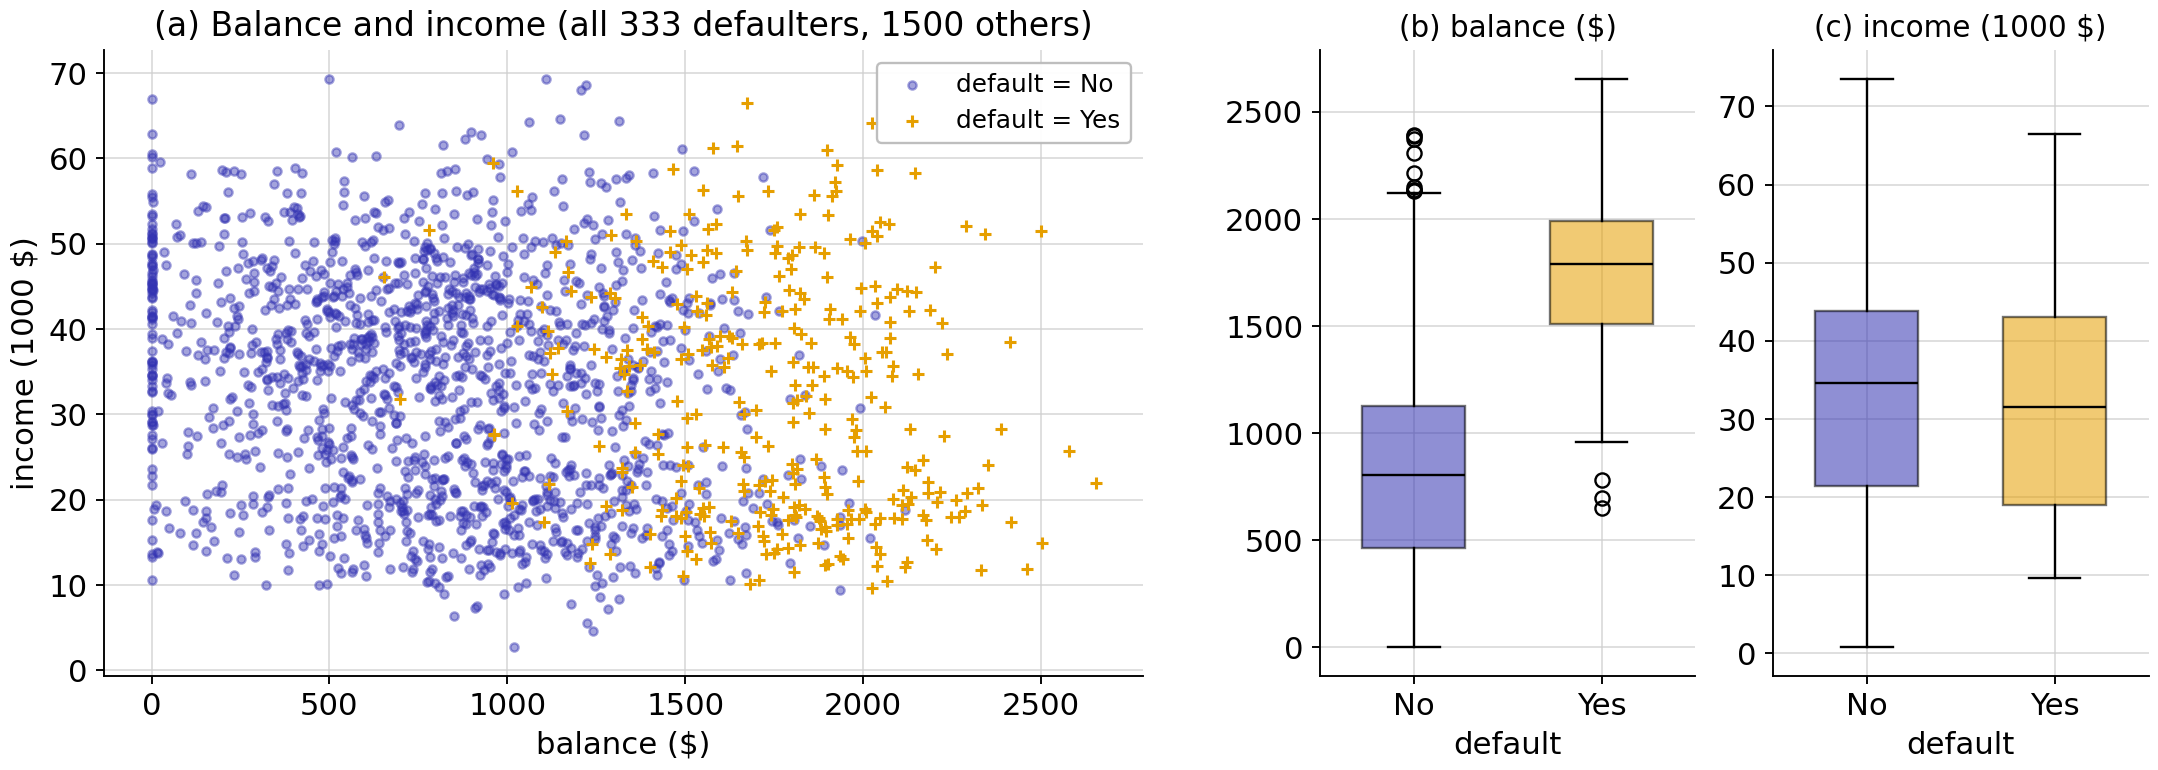
\includegraphics[width=0.97\textwidth,height=0.5\textheight,keepaspectratio]{images/cls_default_data.png}
  \end{center}
  \begin{itemize}\setlength{\itemsep}{2pt}
    \item $n=10\,000$ customers, of which only $333$ ($3.33\,\%$) defaulted.
    \item Defaulters have clearly \textbf{higher balances}; income hardly
          differs between the groups.
  \end{itemize}
  \sourcenote{Default data from James, Witten, Hastie, Tibshirani: \emph{An Introduction to Statistical Learning}, www.statlearning.com}
\end{frame}

\subsection{Two-way tables and conditional probability}

\begin{frame}{Default by student status -- a two-way table}
  \guidingquestion{Do students default more often than non-students? Before
  building a model, we simply \textbf{count}.}
  \begin{columns}[T]
    \begin{column}{0.49\textwidth}
      \centering
      \textbf{Counts} $n(\cdot)$\\[2pt]
      \renewcommand{\arraystretch}{1.15}
      \begin{tabular}{@{}l|cc|c@{}}
        \toprule
        & no default & default & Total\\
        \midrule
        non-student & $6850$ & $206$ & $7056$\\
        student & $2817$ & $127$ & $2944$\\
        \midrule
        Total & $9667$ & $333$ & $10\,000$\\
        \bottomrule
      \end{tabular}
    \end{column}
    \begin{column}{0.49\textwidth}
      \centering
      \textbf{Relative frequencies} $n(\cdot)/n$\\[2pt]
      \renewcommand{\arraystretch}{1.15}
      \begin{tabular}{@{}l|cc|c@{}}
        \toprule
        & no default & default & Total\\
        \midrule
        non-student & $0.6850$ & $0.0206$ & $\mathbf{0.7056}$\\
        student & $0.2817$ & \textcolor{hsbiorange!85!black}{$\mathbf{0.0127}$} & $\mathbf{0.2944}$\\
        \midrule
        Total & $\mathbf{0.9667}$ & $\mathbf{0.0333}$ & $1$\\
        \bottomrule
      \end{tabular}
    \end{column}
  \end{columns}
  \medskip
  \begin{itemize}\setlength{\itemsep}{2pt}
    \item \textbf{Joint} relative frequency (inner cells): \textcolor{hsbiorange!85!black}{$1.27\,\%$}
          of all customers are students \emph{and} defaulted.
    \item \textbf{Marginal} relative frequencies (\textbf{bold} totals): $29.44\,\%$
          are students, $3.33\,\%$ defaulted -- each variable on its own.
  \end{itemize}
\end{frame}

\begin{frame}{Conditional relative frequencies -- change the denominator}
  \begin{block}{``Among the students, what share defaulted?''}
    Look only at the row ``student'' and divide by \emph{its} total:
    \[
      \frac{n(\text{student}\cap\text{default})}{n(\text{student})}
      =\frac{127}{2944}=0.0431
      \qquad\Bigl(=\frac{0.0127}{0.2944}=\frac{\text{joint}}{\text{marginal}}\Bigr)
    \]
  \end{block}
  \begin{columns}[c]
    \begin{column}{0.47\textwidth}
      \centering
      \renewcommand{\arraystretch}{1.12}
      \begin{tabular}{@{}l|cc|c@{}}
        \toprule
        & no default & default & Total\\
        \midrule
        non-student & $0.9708$ & $\mathbf{0.0292}$ & $1$\\
        student & $0.9569$ & $\mathbf{0.0431}$ & $1$\\
        \midrule
        all customers & $0.9667$ & $0.0333$ & $1$\\
        \bottomrule
      \end{tabular}\\[1pt]
      {\footnotesize each row divided by its row total}
    \end{column}
    \begin{column}{0.51\textwidth}
      \small
      \begin{itemize}\setlength{\itemsep}{3pt}
        \item Students default \textbf{more often}: $4.31\,\%$ vs.\ $2.92\,\%$
              (overall $3.33\,\%$).
        \item The other direction is a \emph{different} question:
              $\frac{127}{333}=0.381$ -- $38\,\%$ of the \emph{defaulters}
              are students (divide by the column total).
      \end{itemize}
    \end{column}
  \end{columns}
  \smallskip
  \inworten{Conditioning = restricting attention to one row (or column)
  and dividing by its total.}
\end{frame}

\begin{frame}{Conditional probability -- definition and two rules}
  \begin{block}{Conditional probability of $A$ given $B$}
    \vspace{-0.2em}
    \[
      P(A\mid B)=\frac{P(A\cap B)}{P(B)}\qquad(P(B)>0)
    \]
  \end{block}
  \inworten{the share of the cases in $B$ that also belong to $A$ (a row or
  column share of the table).}
  \smallskip
  \begin{columns}[T]
    \begin{column}{0.49\textwidth}
      \begin{block}{Multiplication rule (``$A$ and $B$'')}
        \centering
        $P(A\cap B)=P(A\mid B)\,P(B)=P(B\mid A)\,P(A)$
      \end{block}
    \end{column}
    \begin{column}{0.49\textwidth}
      \begin{block}{Addition rule (``$A$ or $B$'')}
        \centering
        $P(A\cup B)=P(A)+P(B)-P(A\cap B)$
      \end{block}
    \end{column}
  \end{columns}
  \begin{exampleblock}{Default data ($A=$ default, $B=$ student)}
    $P(A\mid B)=0.0127/0.2944=0.0431$; \ and back:
    $P(A\cap B)=0.0431\cdot0.2944=0.0127$.\\
    $P(A\cup B)=0.0333+0.2944-0.0127=0.3150$: $31.5\,\%$ are students
    \emph{or} defaulters (or both).
  \end{exampleblock}
  {\footnotesize Relative frequencies in the data \emph{estimate} these
  probabilities, e.g.\ $\hat P(\text{default}\mid\text{student})=0.0431$.\par}
\end{frame}

\begin{frame}{Independence}
  \begin{block}{Definition}
    Two events $A$ and $B$ are \textbf{independent} if
    \vspace{-0.3em}
    \[
      P(A\cap B)=P(A)\,P(B)
      \qquad\Longleftrightarrow\qquad
      P(A\mid B)=P(A)\quad(P(B)>0).
    \]
  \end{block}
  \inworten{knowing that $B$ occurred does not change the probability of $A$.}
  \begin{exampleblock}{Default data: are default and student status independent?}
    $P(\text{default})\,P(\text{student})=0.0333\cdot0.2944=0.0098
    \neq0.0127=P(\text{default}\cap\text{student})$\\
    $\Rightarrow$ \textbf{not independent}; equivalently
    $P(\text{default}\mid\text{student})=0.0431\neq0.0333$.\\
    Independence would mean $10\,000\cdot0.0098=98$ student defaulters --
    we observe $127$.
  \end{exampleblock}
  \kernaussage{If $Y$ were independent of $X$, knowing $X$ would not help to
  predict $Y$: classification lives on the \textbf{dependence} of $Y$ on $X$.}
\end{frame}

\begin{frame}{Classification = estimating $P(Y=1\mid x)$}
  \begin{itemize}\setlength{\itemsep}{2pt}
    \item For a \textbf{categorical} $x$ (student yes/no) the two-way table
          gives $\hat P(\text{default}\mid x)$ directly.
    \item \textbf{Balance} is metric: almost every customer has a different
          value. A first attempt -- group the balances into classes:
  \end{itemize}
  \begin{center}
    \renewcommand{\arraystretch}{1.1}
    \begin{tabular}{@{}lccccc@{}}
      \toprule
      balance class (\$) & $[0,500)$ & $[500,1000)$ & $[1000,1500)$ & $[1500,2000)$ & $\ge2000$\\
      \midrule
      customers & $2613$ & $3755$ & $2721$ & $805$ & $106$\\
      defaulters & $0$ & $6$ & $69$ & $177$ & $81$\\
      default rate $\hat P(\text{default}\mid\text{class})$ & $0.000$ & $0.002$ & $0.025$ & $0.220$ & $0.764$\\
      \bottomrule
    \end{tabular}
  \end{center}
  \inworten{The conditional default rate first hardly moves, then rises
  steeply -- an \textbf{S-shape}. But the classes are crude: a customer with
  $1999$\,\$ is treated like one with $1500$\,\$.}
  \kernaussage{Classification means estimating the \textbf{conditional
  probability} $p(x)=P(Y=1\mid X=x)$ as a smooth function of $x$ -- this needs
  a \textbf{model}.}
\end{frame}

\begin{frame}[fragile]{Two-way tables with Python}
\begin{lstlisting}
import pandas as pd
df = pd.read_csv("../data/Default.csv")                   # n = 10 000 customers
tab = pd.crosstab(df.student, df.default, margins=True)   # counts + totals
print(tab)
print(pd.crosstab(df.student, df.default, normalize="index").round(4))
\end{lstlisting}
  \begin{columns}[T]
    \begin{column}{0.42\textwidth}
\begin{lstlisting}[style=Pyout]
default    No  Yes    All
student
No       6850  206   7056
Yes      2817  127   2944
All      9667  333  10000
default      No     Yes
student
No       0.9708  0.0292
Yes      0.9569  0.0431
\end{lstlisting}
    \end{column}
    \begin{column}{0.56\textwidth}
      \small
      \renewcommand{\arraystretch}{1.2}
      \begin{tabular}{@{}ll@{}}
        \toprule
        \textbf{Option} & \textbf{Result}\\
        \midrule
        \texttt{margins=True} & adds row and column totals\\
        \texttt{normalize="all"} & joint relative frequencies\\
        \texttt{normalize="index"} & each \textbf{row} sums to $1$\\
        \texttt{normalize="columns"} & each \textbf{column} sums to $1$\\
        \bottomrule
      \end{tabular}
    \end{column}
  \end{columns}
  \smallskip
  \inworten{\texttt{"index"} conditions on the row variable (student
  status), \texttt{"columns"} on the column variable.}
  \trynotebook{section 1.2 ``Two-way tables and conditional probability''}
\end{frame}

\begin{frame}{Exercise -- newsletter and purchases}
  \begin{block}{Problem statement}
    \begin{columns}[c]
      \begin{column}{0.5\textwidth}
        An online shop records for $n=60$ randomly chosen customers whether
        they subscribe to the newsletter and whether they bought something
        last month.
      \end{column}
      \begin{column}{0.46\textwidth}
        \centering
        \renewcommand{\arraystretch}{1.0}
        \begin{tabular}{@{}l|cc|c@{}}
          \toprule
          newsletter $\backslash$ purchase & yes & no & Total\\
          \midrule
          yes & $15$ & $5$ & $20$\\
          no & $15$ & $25$ & $40$\\
          \midrule
          Total & $30$ & $30$ & $60$\\
          \bottomrule
        \end{tabular}
      \end{column}
    \end{columns}
    \begin{enumerate}
      \item Compute the marginal relative frequencies and the joint one of
            (yes, yes). Are newsletter and purchase independent? How many
            subscribing buyers would independence predict?
      \item Compute the purchase rates of subscribers and of
            non-subscribers and compare them with the overall rate.
      \item Compute the share of subscribers among the buyers. Why does it
            differ from the purchase rate of the subscribers?
    \end{enumerate}
  \end{block}
\end{frame}

\begin{frame}{Solution -- newsletter and purchases}
  \textbf{(1)} Marginal: $\frac{20}{60}=0.333$ subscribe,
  $\frac{40}{60}=0.667$ do not; $\frac{30}{60}=0.5$ buy.
  Joint: $\frac{15}{60}=0.25$.
  \[
    \text{independence would require } 0.333\cdot0.5=0.167
    \;\neq\; 0.25
    \;\Rightarrow\;\textbf{not independent}.
  \]
  Under independence we would expect $60\cdot0.167=10$ subscribers who buy
  -- we observe $15$.

  \medskip
  \textbf{(2)} Condition on the row (divide by the row total):
  \[
    P(\text{purchase}\mid\text{subscriber})=\tfrac{15}{20}=\textbf{0.75},
    \qquad
    P(\text{purchase}\mid\text{non-subscriber})=\tfrac{15}{40}=\textbf{0.375}
  \]
  Subscribers buy twice as often; under independence both rates would equal
  the overall rate $0.5$.

  \medskip
  \textbf{(3)} Condition on the column ``purchase yes'':
  $P(\text{subscriber}\mid\text{purchase})=\frac{15}{30}=\textbf{0.5}$ -- half
  of the buyers subscribe. Same cell ($15$), different denominator: $20$
  subscribers in (2), $30$ buyers in (3).
  \begin{alertblock}{Common mistakes}
    Confusing $P(A\mid B)$ with $P(B\mid A)$ -- and reading the association
    as an effect: loyal customers may simply be more likely to subscribe.
  \end{alertblock}
\end{frame}

\begin{frame}[fragile]{Conditional probability and independence with Python}
  \textbf{Default data:} conditional probability, the two rules,
  independence:
\begin{lstlisting}
d = df.default == "Yes"                    # True for the defaulters
s = df.student == "Yes"                    # True for the students
p_d, p_s, p_ds = d.mean(), s.mean(), (d & s).mean()   # 0.0333  0.2944  0.0127
print(p_ds / p_s)                          # P(default | student) = 0.0431
print(p_ds / p_s * p_s)                    # multiplication rule: back to 0.0127
print(p_d + p_s - p_ds)                    # addition rule: P(default or student) = 0.3150
print(p_d * p_s)                           # 0.0098 != 0.0127 -> not independent
\end{lstlisting}
  \textbf{Default rate by balance class} (slide ``Classification $=$
  estimating $P(Y=1\mid x)$''):
\begin{lstlisting}
import numpy as np
bal_class = pd.cut(df.balance, [0, 500, 1000, 1500, 2000, np.inf], right=False)
print(pd.crosstab(bal_class, df.default, normalize="index").round(3))
# column "Yes": 0.000  0.002  0.025  0.220  0.764 -- the S-shape
\end{lstlisting}
  \inworten{the mean of a True/False column is the share of \texttt{True}
  values; \texttt{d \& s} means ``$A$ and $B$''.}
  \trynotebook{section 1.2 ``Two-way tables and conditional probability''}
\end{frame}

\begin{frame}{Exercise -- streaming and gaming (exam style)}
  \begin{block}{Problem statement}
    Among the users of a smartphone model, $60\,\%$ use the streaming app
    ($S$), $50\,\%$ play games ($G$) and $30\,\%$ do both.
    \begin{enumerate}
      \item Compute $P(G\mid S)$ and interpret it.
      \item Compute $P(S\cup G)$. What share of the users does neither?
      \item Check whether $S$ and $G$ are independent.
      \item Fill in the two-way table of probabilities for $S$/not $S$ and
            $G$/not $G$.
    \end{enumerate}
  \end{block}
\end{frame}

\begin{frame}{Solution -- streaming and gaming (exam style)}
  \begin{columns}[T]
    \begin{column}{0.57\textwidth}
      \textbf{(1)} $\;P(G\mid S)=\frac{P(G\cap S)}{P(S)}=\frac{0.30}{0.60}=\textbf{0.50}$:
      half of the streaming users also play games.

      \medskip
      \textbf{(2)} $\;P(S\cup G)=0.60+0.50-0.30=\textbf{0.80}$;\\
      neither: $1-0.80=\textbf{0.20}$. (Without $-0.30$ the users who do
      both are counted twice: $1.10>1$.)

      \medskip
      \textbf{(3)} $\;P(S)\,P(G)=0.60\cdot0.50=0.30=P(S\cap G)$\\
      $\Rightarrow$ \textbf{independent}. Equivalently
      $P(G\mid S)=0.50=P(G)$: knowing that someone streams does not change
      the probability that they play.
    \end{column}
    \begin{column}{0.41\textwidth}
      \textbf{(4)} Enter the given values, fill the rest by subtraction:
      \begin{center}
        \renewcommand{\arraystretch}{1.15}
        \begin{tabular}{@{}l|cc|c@{}}
          \toprule
          & $G$ & not $G$ & Total\\
          \midrule
          $S$ & $\mathbf{0.30}$ & $0.30$ & $\mathbf{0.60}$\\
          not $S$ & $0.20$ & $0.20$ & $0.40$\\
          \midrule
          Total & $\mathbf{0.50}$ & $0.50$ & $1$\\
          \bottomrule
        \end{tabular}\\[1pt]
        {\footnotesize given values in bold}
      \end{center}
      \begin{alertblock}{Common mistake}
        Independent $\neq$ disjoint: disjoint means $P(S\cap G)=0$ -- here
        $30\,\%$ do both.
      \end{alertblock}
    \end{column}
  \end{columns}
\end{frame}

\subsection{Why not linear regression?}

\begin{frame}{Why not simply use linear regression?}
  \begin{block}{Tempting idea}
    Code $Y=1$ for default and $Y=0$ otherwise and run the regression of
    Part~4: $\hat y=\hat\beta_0+\hat\beta_1\,\text{balance}$.
  \end{block}
  \begin{center}
    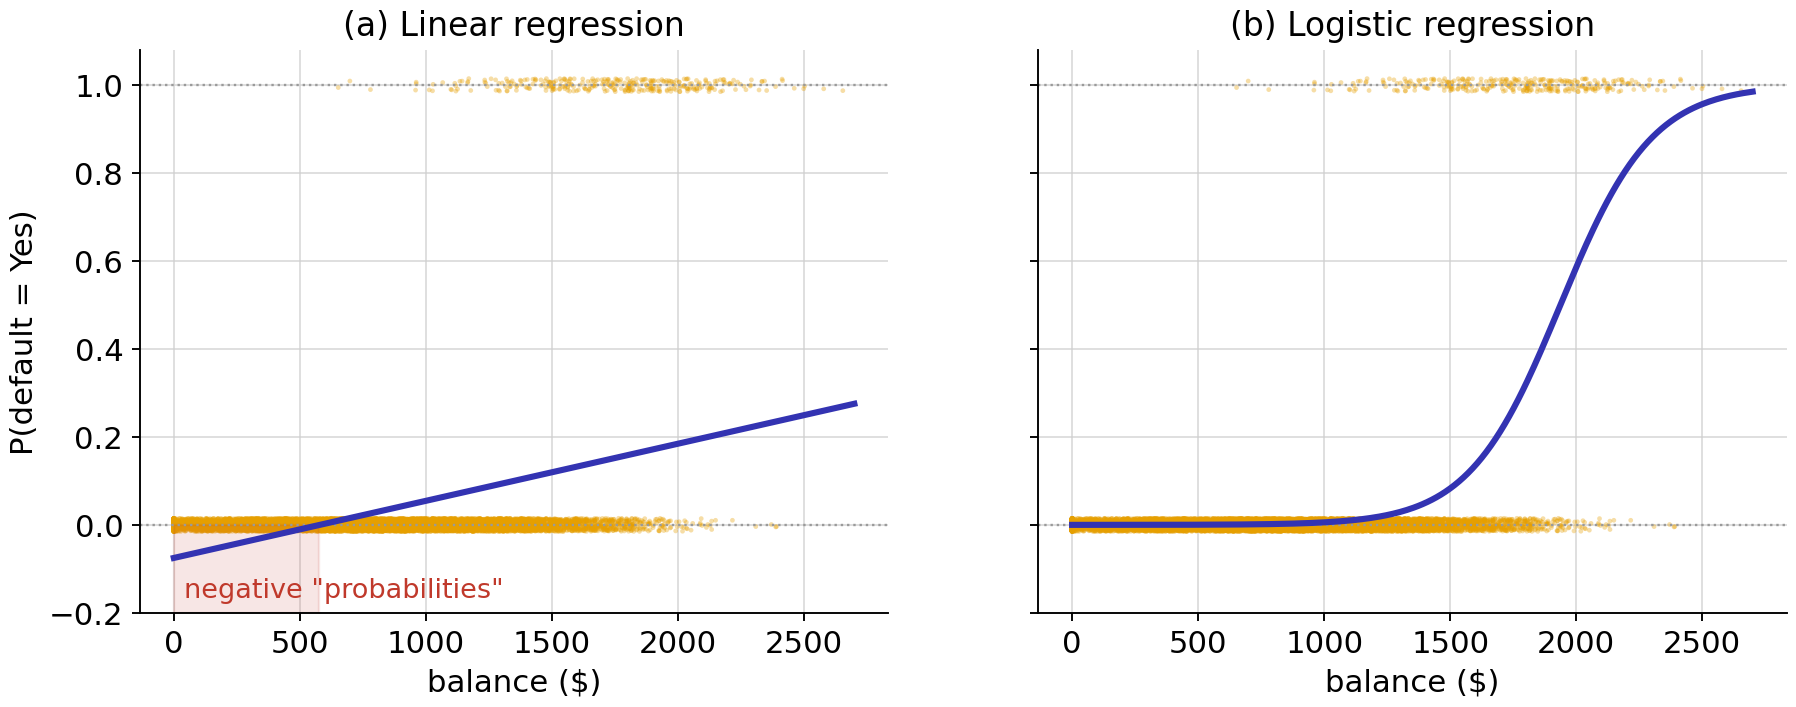
\includegraphics[width=0.9\textwidth,height=0.46\textheight,keepaspectratio]{images/cls_linear_vs_logistic.png}
  \end{center}
  \inworten{The straight line predicts \emph{negative} default
  ``probabilities'' for $3123$ customers (all balances below $579$\,\$); the
  S-curve stays between $0$ and $1$.}
\end{frame}

\begin{frame}{Three problems of linear regression with a $0/1$ variable}
  \begin{alertblock}{Problems}
    \begin{enumerate}\setlength{\itemsep}{3pt}
      \item \textbf{Predictions outside $[0,1]$} -- they cannot be read as
            probabilities.
      \item \textbf{Heteroscedasticity by construction} --
            $\operatorname{Var}(Y\mid x)=p(x)\,(1-p(x))$ depends on $x$, so
            the standard errors and tests of Part~4 are not valid.
      \item \textbf{No natural extension to more than two categories} --
            codes $1,2,3$ would impose an order and equal distances that
            the categories do not have.
    \end{enumerate}
  \end{alertblock}
  \kernaussage{We need a model whose output is always a probability in
  $(0,1)$ -- the \textbf{logistic regression}.}
\end{frame}

\begin{frame}[fragile]{Linear regression on a $0/1$ variable with Python}
\begin{lstlisting}
import statsmodels.formula.api as smf
import matplotlib.pyplot as plt
df["y"] = (df.default == "Yes").astype(int)     # 1 = default, 0 = no
lpm = smf.ols("y ~ balance", data=df).fit()     # the regression of Part 4
print(lpm.params)                               # -0.0752, 0.000130
print((lpm.fittedvalues < 0).sum())             # 3123 negative "probabilities"
print(df.balance[lpm.fittedvalues < 0].max())   # all balances below 579 $
plt.scatter(df.balance, df.y, s=3)              # the 0/1 data
plt.plot(df.balance, lpm.fittedvalues, "r")     # fitted straight line
\end{lstlisting}
  \begin{columns}[T]
    \begin{column}{0.36\textwidth}
\begin{lstlisting}[style=Pyout]
Intercept   -0.075192
balance      0.000130
dtype: float64
3123
578.836277403294
\end{lstlisting}
    \end{column}
    \begin{column}{0.62\textwidth}
      \small
      \begin{itemize}\setlength{\itemsep}{2pt}
        \item $\hat y=-0.0752+0.000130\cdot\text{balance}<0$ for every
              balance below $0.0752/0.000130\approx579$\,\$.
        \item Python fits the line without any warning -- checking the
              model is our job.
      \end{itemize}
    \end{column}
  \end{columns}
  \trynotebook{section 1.3 ``Why not linear regression?''}
\end{frame}

\begin{frame}{Exercise -- why not linear regression?}
  \begin{block}{Problem statement}
    A colleague wants to predict the emergency diagnosis of a patient. She
    codes the three \emph{unordered} categories as $Y=1$ (stroke), $Y=2$
    (overdose), $Y=3$ (seizure) and fits a linear regression.
    \begin{enumerate}
      \item Which implicit assumptions does the coding $1,2,3$ make?
      \item With only two categories coded $0/1$: name two problems of the
            fitted values as probabilities.
      \item Would relabelling the categories change the fit? What does this
            imply?
    \end{enumerate}
  \end{block}
\end{frame}

\begin{frame}{Solution -- why not linear regression?}
  \begin{enumerate}\setlength{\itemsep}{4pt}
    \item \textbf{Order and equal spacing:} the coding claims stroke $<$
          overdose $<$ seizure and equal distances between them. A fitted
          value of $1.5$ would mean ``halfway between stroke and overdose''
          -- medically meaningless.
    \item \textbf{Two problems:} fitted values can lie outside $[0,1]$
          (e.g.\ a negative probability), and the error variance
          $p(1-p)$ is not constant.
    \item \textbf{Yes:} swapping the codes of stroke and seizure gives a
          different response and hence a different fit -- although the data
          are the same. The result depends on an arbitrary choice, so linear
          regression is \emph{not appropriate} here.
  \end{enumerate}
  \begin{alertblock}{Common mistake}
    Hoping that more data fix the problem. The flaw lies in the model
    specification, not in sampling noise.
  \end{alertblock}
\end{frame}

% ============================================================================
% SECTION 2: LOGISTIC REGRESSION
% ============================================================================
\section[Logistic regression]{Logistic Regression}

\subsection{Probability, odds and log-odds}

\begin{frame}{Odds -- another way to express a probability}
  \begin{block}{Definition}
    For an event with probability $p$:
    \[
      \text{odds}=\frac{p}{1-p}\in(0,\infty),
      \qquad
      \text{log-odds (logit)}=\log\frac{p}{1-p}\in(-\infty,\infty).
    \]
  \end{block}
  \begin{center}
    \renewcommand{\arraystretch}{1.25}
    \begin{tabular}{lccccc}
      \toprule
      Probability $p$ & $0.1$ & $0.2$ & $0.5$ & $0.8$ & $0.9$\\
      \midrule
      Odds $p/(1-p)$ & $0.111$ & $0.25$ & $1$ & $4$ & $9$\\
      Log-odds & $-2.197$ & $-1.386$ & $0$ & $1.386$ & $2.197$\\
      \bottomrule
    \end{tabular}
  \end{center}
  \inworten{Odds of $4$ mean ``$4$ to $1$'': the event occurs four times as
  often as it does not ($p=0.8$). Back from odds to probability:
  $p=\text{odds}/(1+\text{odds})$.}
\end{frame}

\begin{frame}{Why log-odds?}
  \begin{center}
    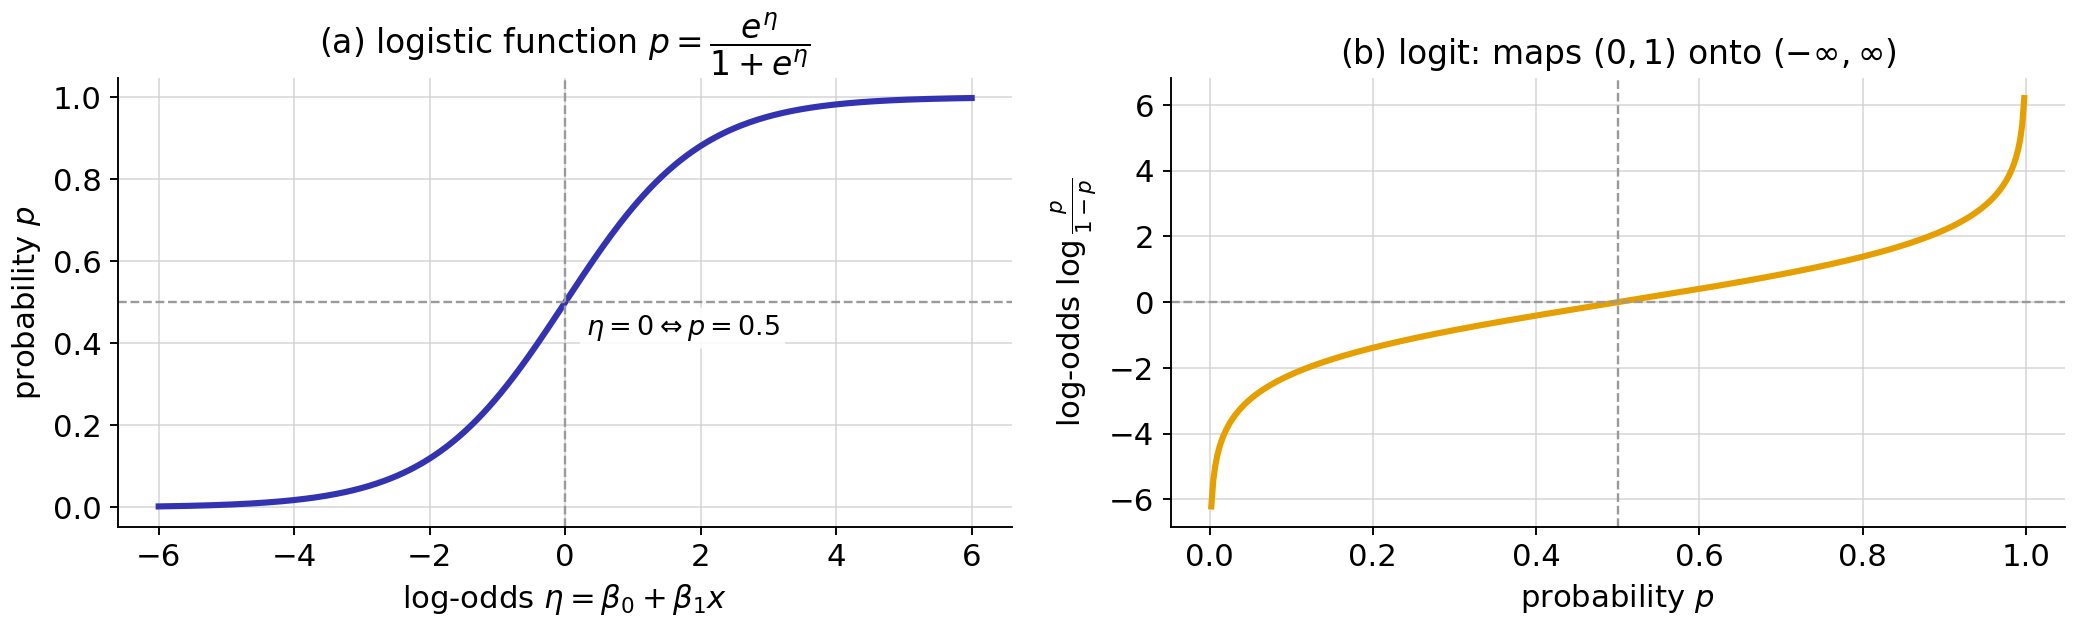
\includegraphics[width=0.95\textwidth,height=0.52\textheight,keepaspectratio]{images/cls_sigmoid.png}
  \end{center}
  \begin{itemize}\setlength{\itemsep}{2pt}
    \item The log-odds can take \textbf{any real value} -- just like the
          right-hand side $\beta_0+\beta_1x$ of a regression.
    \item The logistic function (a) is the inverse of the logit (b): it maps
          every log-odds value back into $(0,1)$.
  \end{itemize}
\end{frame}

\begin{frame}[fragile]{Odds and log-odds with Python}
\begin{lstlisting}
p = np.array([0.1, 0.2, 0.5, 0.8, 0.9])
odds = p / (1 - p)                       # 0.111  0.25  1  4  9
logodds = np.log(odds)                   # natural log: -2.197 ... 2.197
print(pd.DataFrame({"p": p, "odds": odds, "logodds": logodds}).round(3))
print(odds / (1 + odds))                 # back to p: 0.1 0.2 0.5 0.8 0.9
eta = np.linspace(-6, 6, 200)            # a grid of log-odds values
plt.plot(eta, np.exp(eta) / (1 + np.exp(eta)))   # logistic function, panel (a)
\end{lstlisting}
  \begin{columns}[T]
    \begin{column}{0.34\textwidth}
\begin{lstlisting}[style=Pyout]
     p   odds  logodds
0  0.1  0.111   -2.197
1  0.2  0.250   -1.386
2  0.5  1.000    0.000
3  0.8  4.000    1.386
4  0.9  9.000    2.197
\end{lstlisting}
    \end{column}
    \begin{column}{0.64\textwidth}
      \small
      \begin{itemize}\setlength{\itemsep}{2pt}
        \item The same table as on the slide ``Odds'' -- every operation
              works element by element on the whole array.
        \item \texttt{np.log} is the \textbf{natural} logarithm (base $e$),
              \texttt{np.exp} its inverse.
        \item \texttt{np.exp(eta) / (1 + np.exp(eta))} turns log-odds into a
              probability -- we need it again for $\hat p(x)$.
      \end{itemize}
    \end{column}
  \end{columns}
  \trynotebook{section 2.1 ``Probability, odds and log-odds''}
\end{frame}

\begin{frame}{Exercise -- probability, odds and log-odds}
  \begin{block}{Problem statement}
    In the two-way table of Section~1, $127$ of the $2944$ students and $206$
    of the $7056$ non-students defaulted.
    \begin{enumerate}
      \item Compute the probability, the odds and the log-odds of default
            for students and for non-students.
      \item Compute the \textbf{odds ratio} (odds of the students divided by
            the odds of the non-students) and its logarithm. Interpret it.
      \item Compare the odds ratio with the ratio of the two default
            probabilities. Why are the two so close here?
      \item A churn model assigns a customer the log-odds $-1$. Compute the
            odds and the churn probability.
    \end{enumerate}
  \end{block}
\end{frame}

\begin{frame}{Solution -- probability, odds and log-odds}
  \textbf{(1)} Odds $=$ number of ``yes'' / number of ``no'' -- straight
  from the table:
  \begin{center}
    \renewcommand{\arraystretch}{1.15}
    \begin{tabular}{@{}lccc@{}}
      \toprule
      & probability $p$ & odds $p/(1-p)$ & log-odds $\log(\text{odds})$\\
      \midrule
      students & $127/2944=0.0431$ & $127/2817=0.0451$ & $-3.099$\\
      non-students & $206/7056=0.0292$ & $206/6850=0.0301$ & $-3.504$\\
      \bottomrule
    \end{tabular}
  \end{center}
  \textbf{(2)} Odds ratio $=0.0451/0.0301=\textbf{1.50}$, \ $\log1.50=-3.099-(-3.504)=\textbf{0.405}$:
  the odds of default of students are $1.5$ times (i.e.\ $50\,\%$ higher
  than) those of non-students.

  \medskip
  \textbf{(3)} Probability ratio $0.0431/0.0292=1.48\approx1.50$: for
  \emph{rare} events $1-p\approx1$, so odds $\approx$ probability. For common
  events they differ: $p=0.8$ vs.\ $0.5$ gives a probability ratio of $1.6$
  but an odds ratio of $4/1=4$.

  \medskip
  \textbf{(4)} odds $=e^{-1}=0.368$, \ $p=\dfrac{0.368}{1+0.368}=\textbf{0.269}$.
\end{frame}

\subsection{The model}

\begin{frame}{The logistic regression model}
  \begin{block}{Model: linear on the log-odds scale}
    \[
      \log\frac{p(x)}{1-p(x)}=\beta_0+\beta_1x
      \qquad\Longleftrightarrow\qquad
      p(x)=P(Y=1\mid x)=\frac{e^{\beta_0+\beta_1x}}{1+e^{\beta_0+\beta_1x}}
    \]
  \end{block}
  \begin{itemize}\setlength{\itemsep}{3pt}
    \item Both forms describe the \emph{same} model: the left one shows the
          linearity, the right one guarantees $0<p(x)<1$.
    \item We write $\eta=\beta_0+\beta_1x$ for the \textbf{linear predictor}
          (the log-odds).
    \item Several explanatory variables: $\eta=\beta_0+\beta_1x_1+\dots+\beta_px_p$
          (Section~3).
  \end{itemize}
  \kernaussage{Logistic regression = the regression model of Part~4, applied
  to the \textbf{log-odds} instead of $Y$ itself.}
\end{frame}

\begin{frame}{Reading the model symbol by symbol}
  \begin{center}
    \renewcommand{\arraystretch}{1.3}
    \begin{tabular}{@{}cl@{}}
      \toprule
      \textbf{Symbol} & \textbf{Meaning} \\
      \midrule
      $Y$ & Binary response, $0$ or $1$ (default no/yes) \\
      $p(x)$ & $P(Y=1\mid x)$, the probability of default given $x$ \\
      $p(x)/(1-p(x))$ & The \emph{odds} of default \\
      $\eta=\log[p/(1-p)]$ & The \emph{log-odds}, linear in $x$ \\
      $\beta_1$ & Change of the \emph{log-odds} per unit of $x$ \\
      $e^{\beta_1}$ & Factor by which the \emph{odds} change per unit of $x$ \\
      \bottomrule
    \end{tabular}
  \end{center}
  \inworten{Every probability statement goes through the pipeline
  $x\;\xrightarrow{\ \text{linear}\ }\;\eta\;\xrightarrow{\ \exp\ }\;\text{odds}
  \;\xrightarrow{\ \text{odds}/(1+\text{odds})\ }\;p$.}
\end{frame}

\subsection{Estimation}

\begin{frame}{Estimation: maximum likelihood}
  \begin{block}{Idea}
    Least squares makes no sense for $0/1$ data. Instead we choose the
    coefficients under which the \textbf{observed outcomes are most
    probable}.
  \end{block}
  \begin{block}{Likelihood}
    \[
      L(\beta_0,\beta_1)=\prod_{i:\,y_i=1}p(x_i)\;\prod_{i:\,y_i=0}\bigl(1-p(x_i)\bigr)
    \]
    Each defaulter contributes $p(x_i)$, each non-defaulter $1-p(x_i)$.
  \end{block}
  \begin{itemize}\setlength{\itemsep}{2pt}
    \item In practice we maximise the \textbf{log-likelihood}
          $\log L=\sum_i\bigl[y_i\log p(x_i)+(1-y_i)\log(1-p(x_i))\bigr]$.
    \item There is no closed formula -- Python solves it numerically
          (\texttt{smf.logit(...).fit()}).
  \end{itemize}
\end{frame}

\begin{frame}{Exercise -- which parameters are more plausible?}
  \begin{block}{Problem statement}
    Four customers with balances $1000$, $1500$, $2000$, $2500$\,\$; the last
    two defaulted ($y=0,0,1,1$). Compare two candidate parameter sets:
    \[
      \text{(A)}\ \ \beta_0=-10.65,\ \beta_1=0.0055
      \qquad\qquad
      \text{(B)}\ \ \beta_0=-5,\ \beta_1=0.002
    \]
    \begin{enumerate}
      \item Compute $p(x_i)$ for all four customers under (A) and (B).
      \item Compute the likelihood $L$ for (A) and (B).
      \item Which parameter set would maximum likelihood prefer?
    \end{enumerate}
  \end{block}
\end{frame}

\begin{frame}{Solution (1/2) -- which parameters are more plausible?}
  Example: $\eta(2000)=-10.65+0.0055\cdot2000=0.35$,
  $p=e^{0.35}/(1+e^{0.35})=0.5866$.
  \begin{center}
    \small
    \renewcommand{\arraystretch}{1.08}
    \begin{tabular}{c|c|cc|cc}
      \toprule
      & & \multicolumn{2}{c|}{\textbf{(A)}} & \multicolumn{2}{c}{\textbf{(B)}}\\
      balance & $y_i$ & $p(x_i)$ & contribution & $p(x_i)$ & contribution\\
      \midrule
      $1000$ & $0$ & $0.0058$ & $0.9942$ & $0.0474$ & $0.9526$\\
      $1500$ & $0$ & $0.0832$ & $0.9168$ & $0.1192$ & $0.8808$\\
      $2000$ & $1$ & $0.5866$ & $0.5866$ & $0.2689$ & $0.2689$\\
      $2500$ & $1$ & $0.9569$ & $0.9569$ & $0.5000$ & $0.5000$\\
      \midrule
      \multicolumn{2}{c|}{$L$ (product)} & \multicolumn{2}{c|}{\textbf{0.5117}} & \multicolumn{2}{c}{$0.1128$}\\
      \bottomrule
    \end{tabular}
  \end{center}
  \begin{exampleblock}{Decision}
    Under (A) the observed pattern is $4.5$ times as probable as under (B)
    $\Rightarrow$ maximum likelihood prefers \textbf{(A)}: high probabilities
    for the actual defaulters, low ones for the others.
  \end{exampleblock}
\end{frame}

\begin{frame}[fragile]{Solution (2/2) -- which parameters are more plausible?}
  \textbf{The same calculation in Python} -- one function, two parameter sets:
\begin{lstlisting}
x = np.array([1000, 1500, 2000, 2500]); y = np.array([0, 0, 1, 1])
def likelihood(b0, b1):
    p = np.exp(b0 + b1 * x) / (1 + np.exp(b0 + b1 * x))   # p(x_i)
    return np.prod(np.where(y == 1, p, 1 - p))            # product of contributions
print(likelihood(-10.65, 0.0055))      # (A) 0.5117
print(likelihood(-5, 0.002))           # (B) 0.1128
print(np.log(likelihood(-10.65, 0.0055)))   # log-likelihood of (A): -0.6701
\end{lstlisting}
  \begin{itemize}\setlength{\itemsep}{3pt}
    \item \texttt{np.where(y == 1, p, 1 - p)}: each defaulter contributes
          $p(x_i)$, each non-defaulter $1-p(x_i)$ -- the formula of the
          likelihood slide.
    \item Maximum likelihood searches \emph{all} pairs $(\beta_0,\beta_1)$
          for the largest $L$ (in practice: the largest $\log L$).
          \texttt{smf.logit} does this numerically -- next slide.
  \end{itemize}
  \trynotebook{section 2.3 ``Estimation''}
\end{frame}

\begin{frame}[fragile]{Logistic regression with Python}
  \begin{block}{Fitting the model}
\begin{lstlisting}
import statsmodels.formula.api as smf
df = pd.read_csv("../data/Default.csv")
df["y"] = (df.default == "Yes").astype(int)     # 1 = default, 0 = no
g1 = smf.logit("y ~ balance", data=df).fit(disp=0)
print(g1.summary2().tables[1])
\end{lstlisting}
  \end{block}
\begin{lstlisting}[style=Pyout]
               Coef.  Std.Err.          z          P>|z|     [0.025    0.975]
Intercept -10.651331  0.361169 -29.491287  3.723665e-191 -11.359208 -9.943453
balance     0.005499  0.000220  24.952404  2.010855e-137   0.005067  0.005931
\end{lstlisting}
  \begin{itemize}\setlength{\itemsep}{2pt}
    \item \texttt{smf.logit} fits a logistic regression by maximum
          likelihood ($y$ coded $0/1$): $\hat\eta=-10.65+0.0055\cdot\text{balance}$.
    \item The output looks like \texttt{smf.ols} -- with $z$- instead of
          $t$-values (see ``Inference'').
  \end{itemize}
  \trynotebook{section 2.3 ``Estimation''}
\end{frame}

\subsection{Interpretation}

\begin{frame}{Interpreting the coefficients -- three scales}
  \begin{block}{Three ways to read $\hat\beta_1$}
    \begin{description}\setlength{\itemsep}{3pt}
      \item[Sign:] $\hat\beta_1>0$ $\Rightarrow$ a larger $x$ raises the
            probability of $Y=1$; $\hat\beta_1<0$ lowers it.
      \item[Log-odds:] one unit more of $x$ changes the log-odds by
            $\hat\beta_1$ -- constant, but hard to imagine.
      \item[Odds:] one unit more of $x$ \textbf{multiplies the odds} by
            $e^{\hat\beta_1}$ (\textbf{odds ratio}) -- constant and easy to
            communicate.
    \end{description}
  \end{block}
  \begin{alertblock}{Not on the probability scale}
    The change in the \emph{probability} is not constant: it is largest in
    the steep middle of the S-curve and small at the flat ends.
  \end{alertblock}
  \inworten{Why the odds ratio? $\frac{\text{odds}(x+1)}{\text{odds}(x)}
  =\frac{e^{\beta_0+\beta_1(x+1)}}{e^{\beta_0+\beta_1x}}=e^{\beta_1}$ --
  independent of $x$.}
\end{frame}

\begin{frame}{Worked example: default and balance}
  \textbf{Model:} $\hat\eta=-10.65+0.0055\cdot\text{balance}$.
  \begin{exampleblock}{Three scales for $1000$\,\$ more balance}
    \begin{itemize}\setlength{\itemsep}{3pt}
      \item \textbf{Log-odds:} $+0.0055\cdot1000=+5.5$.
      \item \textbf{Odds:} multiplied by $e^{5.5}\approx245$.
      \item \textbf{Probability:} depends on the starting point:
    \end{itemize}
    \begin{center}
      \renewcommand{\arraystretch}{1.2}
      \begin{tabular}{lcccc}
        \toprule
        balance (\$) & $1000$ & $1500$ & $2000$ & $2500$\\
        \midrule
        $\hat p(x)$ & $0.006$ & $0.083$ & $0.587$ & $0.957$\\
        \bottomrule
      \end{tabular}
    \end{center}
  \end{exampleblock}
  \begin{alertblock}{Common mistake}
    ``The odds multiply by $245$'' does \emph{not} mean the probability is
    $245$ times as large -- probabilities can never exceed $1$.
  \end{alertblock}
\end{frame}

\begin{frame}[fragile]{Odds ratios and predicted probabilities with Python}
\begin{lstlisting}
print(np.exp(g1.params["balance"]))           # odds ratio per 1 $:     1.0055
print(np.exp(1000 * g1.params["balance"]))    # odds ratio per 1000 $:  244.4
new = pd.DataFrame({"balance": [1000, 1500, 2000, 2500]})
eta = g1.predict(new, which="linear")         # log-odds: -5.152 -2.403 0.347 3.096
print(np.exp(eta) / (1 + np.exp(eta)))        # by hand:  0.0058 0.0829 0.5858 0.9567
print(g1.predict(new))                        # the same probabilities in one step
\end{lstlisting}
  \begin{itemize}\setlength{\itemsep}{3pt}
    \item \texttt{new} needs a column with the \textbf{same name} as in the
          formula (\texttt{balance}); one row per customer.
    \item \texttt{which="linear"} returns the log-odds $\hat\eta$; without it,
          \texttt{predict} returns $\hat p(x)$ -- the pipeline
          $x\to\hat\eta\to\hat p$.
    \item Python uses the unrounded coefficients: odds ratio $244.4$ instead
          of $e^{5.5}\approx245$; the probabilities agree with the table of
          the worked example.
  \end{itemize}
  \trynotebook{section 2.4 ``Interpretation''}
\end{frame}

\begin{frame}{Exercise -- computing $\hat p(x)$ from the coefficients}
  \begin{block}{Problem statement}
    The logistic regression of default on balance gives
    $\hat\eta=-10.65+0.0055\cdot\text{balance}$. For a customer with a
    balance of $1500$\,\$:
    \begin{enumerate}
      \item Compute the log-odds $\hat\eta$.
      \item Compute the probability of default $\hat p$.
      \item Compute the odds and relate them to part (1).
      \item At which balance does the model give $\hat p=0.5$?
    \end{enumerate}
  \end{block}
\end{frame}

\begin{frame}{Solution -- computing $\hat p(x)$ from the coefficients}
  \begin{exampleblock}{(1)--(3) Log-odds, probability, odds}
    \[
      \hat\eta = -10.65+0.0055\cdot1500=-2.40,\qquad
      \hat p = \frac{e^{-2.40}}{1+e^{-2.40}}=\frac{0.0907}{1.0907}=\textbf{0.083},
    \]
    \[
      \text{odds} = \frac{0.083}{0.917}=0.091=e^{-2.40}\ \checkmark
      \quad\text{(about one default per eleven non-defaults)}
    \]
  \end{exampleblock}
  \begin{exampleblock}{(4) Balance with $\hat p=0.5$}
    $\hat p=0.5\Leftrightarrow\text{odds}=1\Leftrightarrow\hat\eta=0$:\\
    $0=-10.65+0.0055\cdot\text{balance}$ $\Rightarrow$
    balance $=10.65/0.0055\approx\textbf{1936}$\,\$.
  \end{exampleblock}
  \begin{alertblock}{Common mistake}
    Reading $\hat\eta=-2.40$ as a probability -- log-odds must first be
    passed through the logistic function.
  \end{alertblock}
\end{frame}

\subsection{Inference for the coefficients}

\begin{frame}{Inference -- the same recipe once more}
  \begin{block}{$z$-test for a coefficient (Wald test)}
    \[
      H_0:\beta_j=0\quad\text{vs.}\quad H_1:\beta_j\neq0,
      \qquad
      Z=\frac{\hat\beta_j}{\mathrm{SE}(\hat\beta_j)}\;\approx\;N(0,1)\ \text{ under }H_0
    \]
    Reject if $|Z|>z_{1-\alpha/2}$ ($1.96$ for $\alpha=0.05$); $p=2\,\Phi(-|Z|)$.
  \end{block}
  \begin{block}{Confidence intervals}
    \[
      \beta_j:\ \ \hat\beta_j\pm z_{1-\alpha/2}\,\mathrm{SE}(\hat\beta_j),
      \qquad
      \text{odds ratio } e^{\beta_j}:\ \ \bigl[e^{\text{lower}},\,e^{\text{upper}}\bigr]
    \]
  \end{block}
  \begin{itemize}\setlength{\itemsep}{2pt}
    \item Why $z$ and not $t$? Maximum likelihood estimators are
          approximately normal for large $n$ -- as for the known-variance
          case of Part~3.
    \item The CI for the odds ratio is obtained by \textbf{exponentiating
          the bounds} -- it is not symmetric around $e^{\hat\beta_j}$.
  \end{itemize}
\end{frame}

\begin{frame}{Inference -- balance and student status}
  \begin{exampleblock}{Balance ($\hat\beta_1=0.005499$, $\mathrm{SE}=0.000220$)}
    \[
      Z=\frac{0.005499}{0.000220}=24.95,\qquad p<0.0001,\qquad
      \text{CI}_{0.95}(\beta_1)=[\,0.005067\,;\,0.005931\,]
    \]
    Per $100$\,\$: odds ratio $e^{0.5499}=1.733$, CI
    $[e^{0.5067};\,e^{0.5931}]=[\,1.660\,;\,1.810\,]$ -- every $100$\,\$ of
    balance raises the odds of default by $66$ to $81\,\%$.
  \end{exampleblock}
  \begin{exampleblock}{Student ($\hat\beta=0.4049$, $\mathrm{SE}=0.1150$), \texttt{default $\sim$ student}}
    \[
      Z=\frac{0.4049}{0.1150}=3.52,\qquad p=0.0004,\qquad
      e^{0.4049}=1.50,\quad \text{CI}=[\,1.20\,;\,1.88\,]
    \]
    Students have $50\,\%$ higher odds of default -- \emph{on their own}
    (more on this in Section~3). With a single dummy the model reproduces
    the two-way table: $\hat\beta_0=-3.504$ is the log-odds of the
    non-students and $1.50$ the odds ratio (exercise on odds).
  \end{exampleblock}
\end{frame}

\begin{frame}[fragile]{Inference with Python}
  \textbf{Balance} ($z$-test and CIs by hand and built in):
\begin{lstlisting}
from scipy import stats
z = g1.params / g1.bse                       # balance: z = 24.95
print(2 * stats.norm.cdf(-abs(z)))           # p = 2 Phi(-|z|) = 2.0e-137 (= g1.pvalues)
print(g1.conf_int())                         # beta +- 1.96 SE: [0.005067, 0.005931]
print(np.exp(100 * g1.conf_int().loc["balance"]))   # OR per 100 $: [1.660, 1.810]
\end{lstlisting}
  \textbf{Student status alone:}
\begin{lstlisting}
g2 = smf.logit("y ~ student", data=df).fit(disp=0)
print(g2.pvalues["student[T.Yes]"])          # p = 0.0004
print(np.exp(g2.params))                     # odds ratio student: 1.50
print(np.exp(g2.conf_int()))                 # its 95 % CI: [1.20, 1.88]
\end{lstlisting}
  \inworten{\texttt{conf\_int()} gives the CI for $\beta_j$;
  \texttt{np.exp} of the bounds gives the CI for the odds ratio
  $e^{\beta_j}$. For $99\,\%$: \texttt{conf\_int(alpha=0.01)}.}
  \trynotebook{section 2.5 ``Inference for the coefficients''}
\end{frame}

\begin{frame}{Exercise -- coefficients on the odds scale}
  \begin{block}{Problem statement}
    The logistic regression of default on balance gives
    $\hat\beta_1=0.0055$ (per \$) with $\mathrm{SE}(\hat\beta_1)=0.00022$.
    \begin{enumerate}
      \item By how much do the \emph{log-odds} change for $500$\,\$ more
            balance?
      \item By which factor do the \emph{odds} change for $500$\,\$ more
            balance?
      \item Test $H_0:\beta_1=0$ at $\alpha=0.05$.
      \item Why can we state a constant effect on the odds but not on the
            probability?
    \end{enumerate}
  \end{block}
\end{frame}

\begin{frame}{Solution -- coefficients on the odds scale}
  \textbf{(1)} $\;\Delta\eta=0.0055\cdot500=\textbf{2.75}$.
  \qquad
  \textbf{(2)} $\;e^{2.75}=\textbf{15.6}$: the odds are about $16$ times as
  large.

  \medskip
  \textbf{(3)} $\;Z=0.0055/0.00022=25.0>1.96$ $\Rightarrow$ reject $H_0$:
  balance is a highly significant predictor.

  \medskip
  \textbf{(4)} The log-odds are linear in $x$, so a fixed $\Delta x$ always
  shifts them by $\beta_1\Delta x$ and multiplies the odds by
  $e^{\beta_1\Delta x}$. The probability is the S-shaped logistic function of
  the log-odds:
  \begin{center}
    \renewcommand{\arraystretch}{1.2}
    \begin{tabular}{lccc}
      \toprule
      start & odds before & odds after ($\times15.6$) & probability after\\
      \midrule
      $p=0.10$ & $0.111$ & $1.74$ & $0.63$ \ ($+53$ points)\\
      $p=0.90$ & $9$ & $141$ & $0.993$ \ ($+9$ points)\\
      \bottomrule
    \end{tabular}
  \end{center}
\end{frame}

% ============================================================================
% SECTION 3: MULTIPLE LOGISTIC REGRESSION
% ============================================================================
\section[Multiple logistic]{Multiple Logistic Regression}

\subsection{The model}

\begin{frame}{Several explanatory variables}
  \begin{block}{Model}
    \[
      \log\frac{p(x)}{1-p(x)}=\beta_0+\beta_1x_1+\beta_2x_2+\dots+\beta_px_p
    \]
  \end{block}
  Everything from Part~4 carries over:
  \begin{itemize}\setlength{\itemsep}{3pt}
    \item $\beta_j$ is the change of the log-odds per unit of $x_j$
          \textbf{holding all other variables fixed}; $e^{\beta_j}$ is the
          corresponding odds ratio.
    \item Qualitative variables enter as \textbf{dummies} (e.g.\
          \texttt{student[T.Yes]} $=1$ for students).
    \item Simple and multiple coefficients can differ completely --
          \textbf{confounding}.
  \end{itemize}
\end{frame}

\begin{frame}[fragile]{Multiple logistic regression with Python}
\begin{lstlisting}
g3 = smf.logit("y ~ balance + income + student", data=df).fit(disp=0)
print(g3.summary().tables[1])
\end{lstlisting}
\begin{lstlisting}[style=Pyout]
==================================================================================
                     coef    std err          z      P>|z|      [0.025      0.975]
----------------------------------------------------------------------------------
Intercept        -10.8690      0.492    -22.079      0.000     -11.834      -9.904
student[T.Yes]    -0.6468      0.236     -2.738      0.006      -1.110      -0.184
balance            0.0057      0.000     24.737      0.000       0.005       0.006
income          3.033e-06    8.2e-06      0.370      0.712    -1.3e-05    1.91e-05
==================================================================================
\end{lstlisting}
  \begin{itemize}\setlength{\itemsep}{2pt}
    \item \textbf{Balance:} highly significant, positive.
    \item \textbf{Income:} not significant given balance and student
          ($p=0.71$).
    \item \textbf{Student:} significant and now \emph{negative}:
          $e^{-0.6468}=0.524$.
  \end{itemize}
  \trynotebook{section 3.1 ``The model''}
\end{frame}

\subsection{Confounding: the student paradox}

\begin{frame}{The student paradox}
  \begin{columns}[T]
    \begin{column}{0.48\textwidth}
      \begin{block}{Alone: \texttt{default $\sim$ student}}
        $\hat\beta_{\text{student}}=+0.405$ ($p=0.0004$)\\
        Students default \emph{more often}:\\ $4.31\,\%$ vs.\ $2.92\,\%$
        (two-way table, Section~1).
      \end{block}
    \end{column}
    \begin{column}{0.48\textwidth}
      \begin{block}{Together with balance and income}
        $\hat\beta_{\text{student}}=-0.647$ ($p=0.006$)\\
        At the \emph{same} balance, students default \emph{less often}.
      \end{block}
    \end{column}
  \end{columns}
  \medskip
  \begin{alertblock}{How can both be true?}
    Students carry \textbf{larger balances} on average ($988$\,\$ vs.\
    $772$\,\$) -- and a large balance is the main risk factor. Balance is a
    \textbf{confounder} of the student effect.
  \end{alertblock}
  \inworten{The same phenomenon as the newspaper budget in Part~4: the
  simple coefficient answers a different question than the multiple one.}
\end{frame}

\begin{frame}{The student paradox visualised}
  \begin{center}
    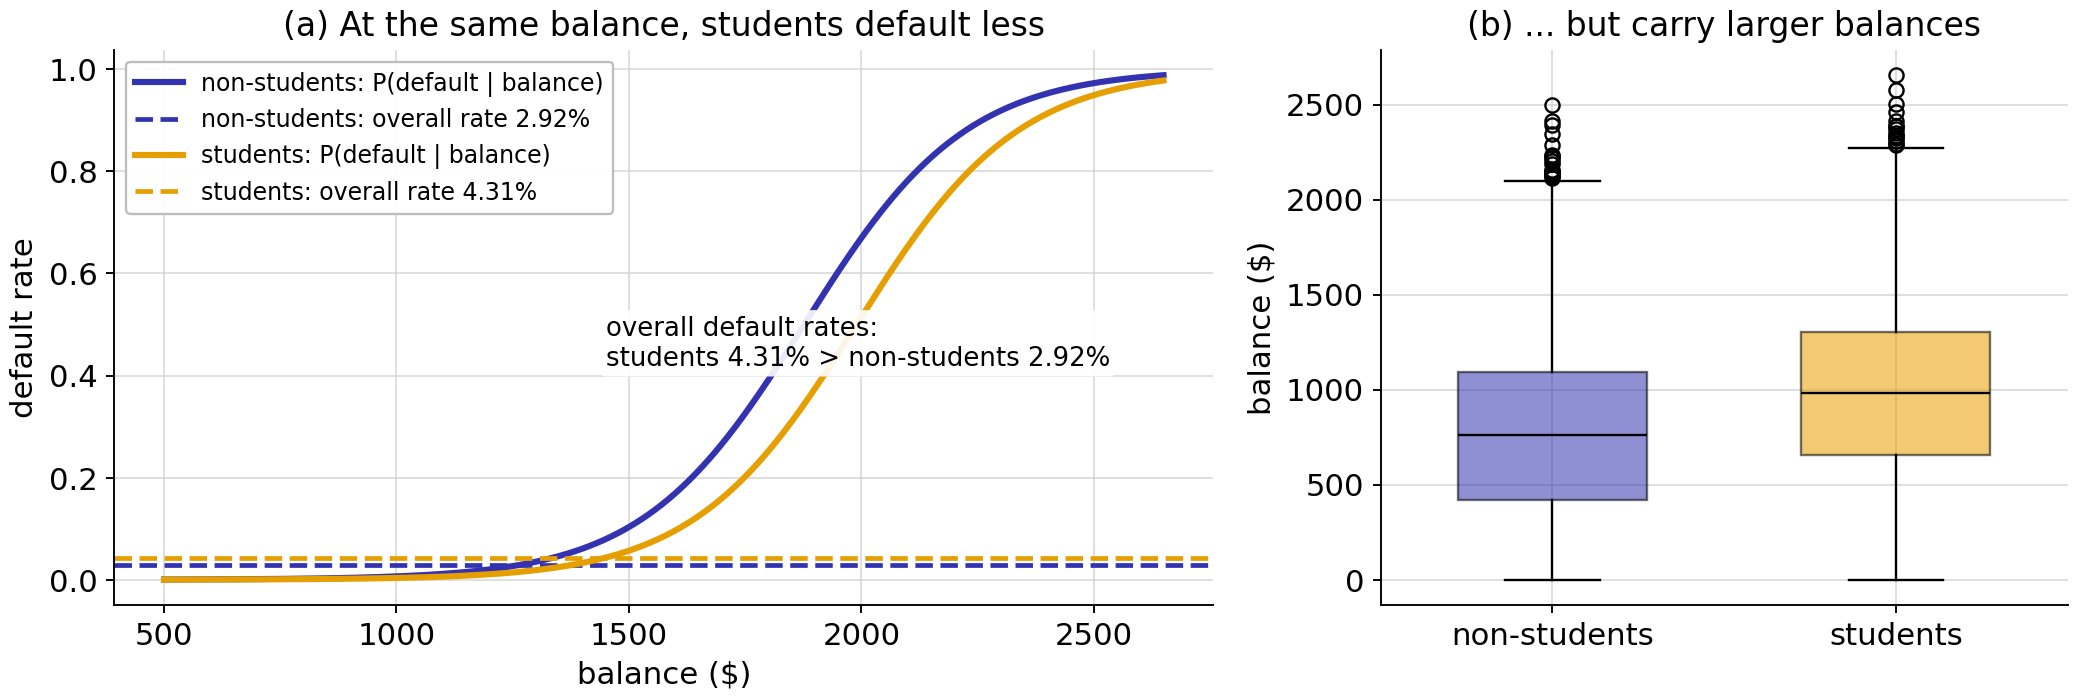
\includegraphics[width=0.95\textwidth,height=0.56\textheight,keepaspectratio]{images/cls_student_paradox.png}
  \end{center}
  \begin{itemize}\setlength{\itemsep}{2pt}
    \item (a) For every balance, the student curve lies \emph{below} the
          non-student curve; the overall rates (dashed) point the other way.
    \item (b) Students are concentrated at higher balances.
  \end{itemize}
\end{frame}

\begin{frame}{Which coefficient is ``right''?}
  \begin{block}{Both -- they answer different questions}
    \begin{itemize}\setlength{\itemsep}{3pt}
      \item \textbf{Simple model:} ``Is a randomly chosen student riskier
            than a randomly chosen non-student?'' -- \emph{yes} (relevant if
            nothing else is known about the applicant).
      \item \textbf{Multiple model:} ``Is a student riskier than a
            non-student \emph{with the same balance and income}?'' --
            \emph{no} (relevant for an individual credit decision, where the
            balance is known).
    \end{itemize}
  \end{block}
  \kernaussage{Always ask \emph{which variables are held fixed} before
  interpreting a coefficient -- in linear and in logistic regression.}
\end{frame}

\begin{frame}[fragile]{The student paradox with Python}
\begin{lstlisting}
print(df.groupby("student").balance.mean())   # No 771.77, Yes 987.82
print(g2.params["student[T.Yes]"])            # alone:              +0.4049
print(g3.params["student[T.Yes]"])            # balance, income too: -0.6468
same = pd.DataFrame({"balance": 1500, "income": 40000, "student": ["No", "Yes"]})
print(g3.predict(same))                       # same balance: 0.1050 vs 0.0579
grid = pd.DataFrame({"balance": np.linspace(500, 2650, 100), "income": 40000})
for st in ["No", "Yes"]:                      # curves as in panel (a)
    plt.plot(grid.balance, g3.predict(grid.assign(student=st)), label=st)
plt.legend()
\end{lstlisting}
  \begin{itemize}\setlength{\itemsep}{3pt}
    \item \textbf{Confounder check:} students carry larger balances
          (\texttt{groupby}), and balance drives default.
    \item \textbf{Same balance and income} ($1500$\,\$, $40\,000$\,\$): a
          non-student defaults with $\hat p=0.105$, a student with only
          $0.058$ -- the multiple model compares like with like.
    \item \texttt{grid.assign(student=st)} sets the student column for all
          rows of the grid.
  \end{itemize}
  \trynotebook{section 3.2 ``Confounding: the student paradox''}
\end{frame}

\subsection{Exercises}

\begin{frame}{Exercise -- inference in the multiple model}
  \begin{block}{Problem statement}
    In the model \texttt{default $\sim$ balance + income + student}:
    \begin{center}
      \renewcommand{\arraystretch}{1.2}
      \begin{tabular}{lcc}
        \toprule
        & $\hat\beta_j$ & $\mathrm{SE}(\hat\beta_j)$\\
        \midrule
        income (per \$) & $3.033\cdot10^{-6}$ & $8.203\cdot10^{-6}$\\
        \texttt{student[T.Yes]} & $-0.6468$ & $0.2363$\\
        \bottomrule
      \end{tabular}
    \end{center}
    \begin{enumerate}
      \item Test $H_0:\beta_{\text{income}}=0$ at $\alpha=0.05$.
      \item Compute a $95\,\%$ CI for the odds ratio of $10\,000$\,\$ more
            income.
      \item Compute the odds ratio for students and its $95\,\%$ CI.
            Interpret it.
    \end{enumerate}
  \end{block}
\end{frame}

\begin{frame}{Solution -- inference in the multiple model}
  \textbf{(1)} $\;Z=\dfrac{3.033}{8.203}=0.37<1.96$ $\Rightarrow$ keep $H_0$
  ($p=0.71$): given balance and student status, income adds no detectable
  information.

  \medskip
  \textbf{(2)} Per $10\,000$\,\$: $\hat\beta=0.0303$, $\mathrm{SE}=0.0820$:
  \[
    0.0303\pm1.96\cdot0.0820=[\,-0.130\,;\,0.191\,]
    \;\Rightarrow\;
    \text{OR}\in[\,e^{-0.130};\,e^{0.191}\,]=[\,0.878\,;\,1.211\,]
  \]
  The interval contains $1$ (``no change of the odds'') -- consistent with (1).

  \medskip
  \textbf{(3)} $e^{-0.6468}=\textbf{0.524}$;
  $-0.6468\pm1.96\cdot0.2363=[\,-1.110\,;\,-0.184\,]$
  $\Rightarrow$ OR $\in[\,0.330\,;\,0.832\,]$.
  \begin{exampleblock}{Interpretation}
    At the same balance and income, a student's odds of default are about
    half ($48\,\%$ lower) those of a non-student; the CI excludes $1$.
  \end{exampleblock}
\end{frame}

\begin{frame}{Exercise -- logistic regression from A to Z}
  \begin{block}{Problem statement}
    Use the multiple model with (rounded) coefficients
    \[
      \hat\eta=-10.869+0.00574\cdot\text{balance}+0.003\cdot\text{income}-0.6468\cdot\text{student}
    \]
    (income in $1000$\,\$, student $=1$ for students). Two customers:
    \begin{itemize}
      \item \textbf{A}: non-student, balance $1000$\,\$, income $40\,000$\,\$;
      \item \textbf{B}: student, balance $2000$\,\$, income $30\,000$\,\$.
    \end{itemize}
    \begin{enumerate}
      \item Compute $\hat\eta$ and $\hat p$ for A and B.
      \item By which factor do the odds change for $100$\,\$ more balance?
      \item At which balance does a non-student with $40\,000$\,\$ income
            reach $\hat p=0.5$? And a student with the same income?
    \end{enumerate}
  \end{block}
\end{frame}

\begin{frame}{Solution (1/2) -- logistic regression from A to Z}
  \begin{exampleblock}{(1) Log-odds and probabilities (watch the units: income in $1000$\,\$)}
    \begin{align*}
      \hat\eta_A&=-10.869+0.00574\cdot1000+0.003\cdot40=-10.869+5.740+0.120=-5.009\\
      \hat\eta_B&=-10.869+0.00574\cdot2000+0.003\cdot30-0.6468=0.054
    \end{align*}
    \[
      \hat p_A=\frac{e^{-5.009}}{1+e^{-5.009}}=\textbf{0.0066},
      \qquad
      \hat p_B=\frac{e^{0.054}}{1+e^{0.054}}=\textbf{0.514}
    \]
    A is a very safe customer, B is right at the knife edge. (Python
    with unrounded coefficients, \texttt{g3.predict(...)}: $0.0066$ and $0.512$.)
  \end{exampleblock}
  \textbf{(2)} $\;e^{0.00574\cdot100}=e^{0.574}=\textbf{1.78}$: $100$\,\$ more
  balance raises the odds by $78\,\%$ -- whatever the starting point.
  \trynotebook{section 3.3 ``Exercises''}
\end{frame}

\begin{frame}{Solution (2/2) -- logistic regression from A to Z}
  \begin{exampleblock}{(3) Decision boundary: $\hat p=0.5\Leftrightarrow\hat\eta=0$}
    Non-student, income $40$:
    \[
      0=-10.869+0.00574\cdot\text{balance}+0.120
      \;\Rightarrow\;
      \text{balance}=\frac{10.869-0.120}{0.00574}\approx\textbf{1873}\,\$
    \]
    Student, income $40$:
    \[
      \text{balance}=\frac{10.869-0.120+0.6468}{0.00574}\approx\textbf{1985}\,\$
    \]
  \end{exampleblock}
  \inworten{A student needs about $0.6468/0.00574\approx113$\,\$ more balance
  to reach the same $50\,\%$ risk -- the negative student coefficient,
  expressed in dollars.}
  \begin{alertblock}{Common mistake}
    Inserting the income in dollars: $0.003\cdot40\,000=120$ would push every
    probability to $1$.
  \end{alertblock}
\end{frame}

% ============================================================================
% SECTION 4: FROM PROBABILITIES TO DECISIONS
% ============================================================================
\section[Decisions]{From Probabilities to Decisions}

\begin{frame}{The classification rule}
  \begin{block}{Rule with threshold $t$}
    \[
      \hat y=\begin{cases}1\ (\text{``default''}) & \text{if } \hat p(x)>t,\\
                         0\ (\text{``no default''}) & \text{otherwise.}\end{cases}
    \]
    The usual default is $t=0.5$: assign the more probable class.
  \end{block}
  \begin{block}{Threshold on the log-odds scale}
    Because the logistic function is increasing,
    \[
      \hat p(x)>t \quad\Longleftrightarrow\quad \hat\eta(x)>\log\frac{t}{1-t}
    \]
    $t=0.5$ corresponds to $\hat\eta>0$; $t=0.2$ to $\hat\eta>\log(0.25)=-1.386$.
  \end{block}
\end{frame}

\begin{frame}{Decision boundary -- default and balance}
  \textbf{Model:} $\hat\eta=-10.65+0.0055\cdot\text{balance}$.
  \begin{center}
    \renewcommand{\arraystretch}{1.4}
    \begin{tabular}{lcc}
      \toprule
      Threshold & log-odds cut-off & balance cut-off\\
      \midrule
      $t=0.5$ & $\hat\eta>0$ & $10.65/0.0055=1936$\,\$\\
      $t=0.2$ & $\hat\eta>\log(0.2/0.8)=-1.386$ & $(10.65-1.386)/0.0055=1684$\,\$\\
      \bottomrule
    \end{tabular}
  \end{center}
  \inworten{Lowering the threshold moves the boundary to the left: more
  defaulters are caught -- but more good customers are rejected as well.}
  \kernaussage{The threshold is not a statistical but a \textbf{business
  decision}: it depends on the cost of a missed defaulter compared with the
  cost of a rejected good customer.}
\end{frame}

\begin{frame}[fragile]{The classification rule with Python}
  \textbf{Decision boundary on the balance scale} (model \texttt{g1}):
\begin{lstlisting}
b0, b1 = g1.params                            # -10.6513, 0.005499
print(-b0 / b1)                               # t = 0.5: boundary 1937 $
print((np.log(0.2 / 0.8) - b0) / b1)          # t = 0.2: boundary 1685 $
\end{lstlisting}
  \textbf{From probabilities to classes:}
\begin{lstlisting}
phat1 = g1.predict(df)                        # P(default) for every customer
yhat = (phat1 > 0.5).astype(int)              # rule: 1 = "default" if p-hat > t
print(yhat.sum(), (phat1 > 0.2).sum())        # flagged: 142 (t = 0.5), 462 (t = 0.2)
\end{lstlisting}
  \begin{itemize}\setlength{\itemsep}{3pt}
    \item Unrounded coefficients: boundaries $1937$ and $1685$\,\$
          (previous slide, rounded: $1936$ and $1684$\,\$).
    \item Lowering $t$ from $0.5$ to $0.2$ flags $462$ instead of $142$
          customers. How many of them really default? $\to$ Section~5.
  \end{itemize}
  \trynotebook{section 4 ``From Probabilities to Decisions''}
\end{frame}

\begin{frame}{Exercise -- from probability to decision}
  \begin{block}{Problem statement}
    Use $\hat\eta=-10.65+0.0055\cdot\text{balance}$. Three applicants have
    balances of $1800$, $2000$ and $2200$\,\$.
    \begin{enumerate}
      \item Compute the predicted probability of default for each.
      \item Classify them with the threshold $t=0.5$.
      \item The bank lowers the threshold to $t=0.2$. Which classifications
            change?
    \end{enumerate}
  \end{block}
\end{frame}

\begin{frame}{Solution -- from probability to decision}
  \begin{exampleblock}{(1) Probabilities}
    \begin{align*}
      1800\colon&\ \ \hat\eta=-10.65+9.90=-0.75, & \hat p&=\tfrac{e^{-0.75}}{1+e^{-0.75}}=0.321\\
      2000\colon&\ \ \hat\eta=-10.65+11.00=\phantom{-}0.35, & \hat p&=\tfrac{e^{0.35}}{1+e^{0.35}}=0.587\\
      2200\colon&\ \ \hat\eta=-10.65+12.10=\phantom{-}1.45, & \hat p&=\tfrac{e^{1.45}}{1+e^{1.45}}=0.810
    \end{align*}
  \end{exampleblock}
  \textbf{(2)} $t=0.5$ (boundary $1936$\,\$): $1800\to$ \textbf{No},
  $2000\to$ \textbf{Yes}, $2200\to$ \textbf{Yes}.

  \medskip
  \textbf{(3)} $t=0.2$ (boundary $1684$\,\$): the applicant with $1800$\,\$
  ($\hat p=0.321>0.2$) flips to \textbf{Yes}; the other two stay
  \textbf{Yes}.

  \medskip
  \inworten{Equally spaced balances ($+200$\,\$) give unequal probability
  steps ($+0.27$, $+0.22$) -- the S-curve is non-linear.}
\end{frame}

% ============================================================================
% SECTION 5: EVALUATING A CLASSIFIER
% ============================================================================
\section[Evaluation]{Evaluating a Classifier}

\subsection{Confusion matrix}

\begin{frame}{Why accuracy alone is not enough}
  \begin{block}{The trivial classifier}
    Only $3.33\,\%$ of the customers default. The ``classifier'' that
    \textbf{always predicts ``no default''} is right for
    $96.67\,\%$ of the customers -- and detects not a single defaulter.
  \end{block}
  \begin{alertblock}{Imbalanced classes}
    With a rare class, a high accuracy is easy to achieve and says little.
    We must look at the two kinds of errors \textbf{separately} -- they also
    have very different costs.
  \end{alertblock}
  \inworten{As in Part~3 there are two ways to be wrong: a false alarm
  (Type~I) and a miss (Type~II).}
\end{frame}

\begin{frame}{The confusion matrix}
  \begin{columns}[c]
    \begin{column}{0.52\textwidth}
      \centering
      \begin{tikzpicture}[font=\small,
          cell/.style={minimum width=2.6cm,minimum height=1.3cm,draw=black!45,align=center}]
        \node[font=\footnotesize\bfseries] at (2.6,3.25) {Predicted};
        \node[font=\footnotesize] at (1.3,2.85) {No};
        \node[font=\footnotesize] at (3.9,2.85) {Yes};
        \node[rotate=90,font=\footnotesize\bfseries] at (-0.75,1.3) {Actual};
        \node[font=\footnotesize] at (-0.3,1.95) {No};
        \node[font=\footnotesize] at (-0.3,0.65) {Yes};
        \node[cell,fill=hsbigruen!18] at (1.3,1.95) {\textbf{TN}\\true negative};
        \node[cell,fill=hsbirot!15]   at (3.9,1.95) {\textbf{FP}\\false positive};
        \node[cell,fill=hsbirot!15]   at (1.3,0.65) {\textbf{FN}\\false negative};
        \node[cell,fill=hsbigruen!18] at (3.9,0.65) {\textbf{TP}\\true positive};
      \end{tikzpicture}
    \end{column}
    \begin{column}{0.46\textwidth}
      \begin{block}{Measures}
        \vspace{-0.6em}
        \begin{align*}
          \text{Accuracy}&=\frac{\mathrm{TP}+\mathrm{TN}}{n}\\[2pt]
          \text{\textcolor{hsbiorange!85!black}{Sensitivity}}&=\frac{\mathrm{TP}}{\mathrm{TP}+\mathrm{FN}}\\[2pt]
          \text{\textcolor{hsbiblau}{Specificity}}&=\frac{\mathrm{TN}}{\mathrm{TN}+\mathrm{FP}}\\[2pt]
          \text{Precision}&=\frac{\mathrm{TP}}{\mathrm{TP}+\mathrm{FP}}
        \end{align*}
      \end{block}
    \end{column}
  \end{columns}
  \medskip
  \begin{itemize}\setlength{\itemsep}{2pt}
    \item \textbf{Sensitivity} (recall): share of actual defaulters that are
          caught. \textbf{Specificity}: share of non-defaulters correctly
          left alone.
    \item \textbf{Precision}: share of flagged customers that really default.
          Error rate $=1-\text{accuracy}$.
  \end{itemize}
\end{frame}

\begin{frame}{Confusion matrix -- Default data, $t=0.5$}
  \textbf{Model:} \texttt{default $\sim$ balance + income + student},
  $t=0.5$, all $n=10\,000$ customers:
  \begin{center}
    \renewcommand{\arraystretch}{1.25}
    \begin{tabular}{l|cc|c}
      \toprule
      & Pred.\ No & Pred.\ Yes & Total\\
      \midrule
      Actual No & $9627$ & $40$ & $9667$\\
      Actual Yes & $228$ & $105$ & $333$\\
      \midrule
      Total & $9855$ & $145$ & $10\,000$\\
      \bottomrule
    \end{tabular}
  \end{center}
  \begin{exampleblock}{Metrics}
    \begin{tabular}{@{}ll@{}}
      Accuracy $=\frac{9627+105}{10\,000}=0.973$ & Sensitivity $=\frac{105}{333}=0.315$\\[4pt]
      Specificity $=\frac{9627}{9667}=0.996$ & Precision $=\frac{105}{145}=0.724$
    \end{tabular}
  \end{exampleblock}
  \inworten{An accuracy of $97.3\,\%$ -- but $228$ of $333$ defaulters
  ($68\,\%$) are missed.}
\end{frame}

\begin{frame}{The confusion matrix is a two-way table}
  Rows: actual class $y$; columns: predicted class $\hat y$. Every measure is
  a relative frequency in this table -- the only question is \textbf{which
  total we divide by}:
  \begin{center}
    \renewcommand{\arraystretch}{1.22}
    \begin{tabular}{@{}llll@{}}
      \toprule
      \textbf{Measure} & \textbf{as a probability} & \textbf{divide by the \ldots} & \textbf{Default, $t=0.5$}\\
      \midrule
      Sensitivity & $P(\hat y=1\mid y=1)$ & row total ``Actual Yes'' & $105/333=0.315$\\
      Specificity & $P(\hat y=0\mid y=0)$ & row total ``Actual No'' & $9627/9667=0.996$\\
      Precision & $P(y=1\mid \hat y=1)$ & column total ``Pred.\ Yes'' & $105/145=0.724$\\
      Accuracy & $P(\hat y=y)$ & grand total $n$ & $9732/10\,000=0.973$\\
      \bottomrule
    \end{tabular}
  \end{center}
  \kernaussage{Sensitivity and precision both count the TP but condition on
  different events: $P(\hat y=1\mid y=1)\neq P(y=1\mid\hat y=1)$ -- like
  $P(\text{default}\mid\text{student})\neq P(\text{student}\mid\text{default})$.}
\end{frame}

\begin{frame}[fragile]{Rates with Python: normalise the rows or the columns}
\begin{lstlisting}
phat = g3.predict(df)                                # P(default = Yes), model g3
pred = phat > 0.5                                    # True = "default" predicted
print(pd.crosstab(df.default, pred, normalize="index").round(4))    # given y
print(pd.crosstab(df.default, pred, normalize="columns").round(4))  # given y-hat
print((pred == df.y).mean())                         # accuracy 0.9732
\end{lstlisting}
  \begin{columns}[T]
    \begin{column}{0.36\textwidth}
\begin{lstlisting}[style=Pyout]
col_0     False   True
default
No       0.9959  0.0041
Yes      0.6847  0.3153
col_0     False   True
default
No       0.9769  0.2759
Yes      0.0231  0.7241
0.9732
\end{lstlisting}
    \end{column}
    \begin{column}{0.62\textwidth}
      \small
      \begin{itemize}\setlength{\itemsep}{3pt}
        \item \textbf{Rows} sum to $1$: row ``Yes'' gives the sensitivity
              $0.3153$ (and the miss rate $0.6847$), row ``No'' the
              specificity $0.9959$.
        \item \textbf{Columns} sum to $1$: column ``True'' gives the
              precision $0.7241$; column ``False'': $97.7\,\%$ of the
              customers predicted ``no default'' really do not default.
        \item \textbf{Accuracy}: the share of customers with $\hat y=y$.
      \end{itemize}
    \end{column}
  \end{columns}
  \trynotebook{section 5.1 ``Confusion matrix''}
\end{frame}

\begin{frame}{Exercise -- reading a confusion matrix}
  \begin{block}{Problem statement}
    The bank lowers the threshold of the same model to $t=0.2$:
    \begin{center}
      \renewcommand{\arraystretch}{1.2}
      \begin{tabular}{l|cc|c}
        \toprule
        & Pred.\ No & Pred.\ Yes & Total\\
        \midrule
        Actual No & $9390$ & $277$ & $9667$\\
        Actual Yes & $130$ & $203$ & $333$\\
        \bottomrule
      \end{tabular}
    \end{center}
    \begin{enumerate}
      \item Compute accuracy, error rate, sensitivity, specificity and
            precision.
      \item Compare with the confusion matrix at $t=0.5$. Which threshold would you
            recommend to the bank?
    \end{enumerate}
  \end{block}
\end{frame}

\begin{frame}{Solution -- reading a confusion matrix}
  \textbf{(1) Metrics at $t=0.2$} (with $t=0.5$ for comparison):
  \begin{center}
    \renewcommand{\arraystretch}{1.15}
    \begin{tabular}{lccl}
      \toprule
      & $t=0.5$ & $t=0.2$ & \\
      \midrule
      Accuracy & $0.973$ & $0.959$ & $=(9390+203)/10\,000$\\
      Error rate & $0.027$ & $0.041$ & $=1-0.959$\\
      Sensitivity & $0.315$ & $0.610$ & $=203/333$\\
      Specificity & $0.996$ & $0.971$ & $=9390/9667$\\
      Precision & $0.724$ & $0.423$ & $=203/(203+277)$\\
      \bottomrule
    \end{tabular}
  \end{center}
  \textbf{(2)} With $t=0.2$ the bank catches almost twice as many defaulters
  ($203$ instead of $105$) at the price of $237$ additional false alarms. If a
  missed default costs much more than a rejected good customer, $t=0.2$ is
  the better choice -- although its accuracy is lower.

  \medskip
  \inworten{Do not confuse sensitivity and precision: both have TP on top, but
  divide by the \emph{actual} ($333$) or the \emph{predicted} ($480$)
  positives.}
\end{frame}

\subsection{Base rates and precision}

\begin{frame}{The base-rate effect}
  \guidingquestion{Our rule with $t=0.2$ catches $61\,\%$ of the defaulters
  and flags only $2.87\,\%$ of the good customers. Are its alarms just as
  reliable in a bank where only $1\,\%$ of the customers default?}
  \begin{columns}[c]
    \begin{column}{0.64\textwidth}
      \centering
      \resizebox{\textwidth}{!}{%
      \begin{tikzpicture}[font=\footnotesize]
        \node[treenode] (r) at (0,0) {$10\,000$\\customers};
        \node[treenodeo] (d) at (3.3,1.15) {$100$ defaulters};
        \node[treenode] (n) at (3.3,-1.15) {$9900$ non-defaulters};
        \node[treenodeo,anchor=west] (dp) at (6.2,1.7) {$\mathbf{61}$ flagged (TP)};
        \node[treenode,anchor=west] (dm) at (6.2,0.6) {$39$ missed (FN)};
        \node[treenodeo,anchor=west] (np) at (6.2,-0.6) {$\mathbf{284}$ flagged (FP)};
        \node[treenode,anchor=west] (nm) at (6.2,-1.7) {$9616$ not flagged (TN)};
        \draw[treeedge] (r.east) -- node[treelab]{$1\,\%$} (d.west);
        \draw[treeedge] (r.east) -- node[treelab]{$99\,\%$} (n.west);
        \draw[treeedge] (d.east) -- node[treelab]{$0.610$} (dp.west);
        \draw[treeedge] (d.east) -- node[treelab]{$0.390$} (dm.west);
        \draw[treeedge] (n.east) -- node[treelab]{$0.0287$} (np.west);
        \draw[treeedge] (n.east) -- node[treelab]{$0.9713$} (nm.west);
      \end{tikzpicture}}
    \end{column}
    \begin{column}{0.34\textwidth}
      \begin{exampleblock}{Precision}
        \[
          \frac{\mathrm{TP}}{\mathrm{TP}+\mathrm{FP}}=\frac{61}{61+284}=\textbf{0.177}
        \]
        Only about one alarm in six -- compared with $0.423$ at the actual
        base rate of $3.33\,\%$.
      \end{exampleblock}
    \end{column}
  \end{columns}
  \medskip
  \inworten{The rule has not changed (same sensitivity and specificity) --
  the mix has: with rare defaulters,
  the few false alarms from the huge majority outnumber the correct alarms.}
\end{frame}

\begin{frame}{Precision depends on the base rate}
  \begin{columns}[c]
    \begin{column}{0.48\textwidth}
      \begin{block}{Precision for base rate $\pi=P(Y=1)$}
        \vspace{-0.3em}
        \[
          \text{precision}=\frac{\text{sens}\cdot\pi}
          {\text{sens}\cdot\pi+(1-\text{spec})(1-\pi)}
        \]
      \end{block}
      \inworten{correct alarms divided by all alarms; false alarms come
      from the $1-\pi$ non-defaulters.}

      \smallskip
      {\small Check ($\pi=0.0333$): $0.610\cdot0.0333=0.0203$,
      $0.0287\cdot0.9667=0.0277$ $\Rightarrow$
      $0.0203/0.0480=0.423$ \checkmark\par}
    \end{column}
    \begin{column}{0.5\textwidth}
      \centering
      \begin{tikzpicture}
        \begin{axis}[width=7.4cm,height=4.7cm,
            xmin=0,xmax=30,ymin=0,ymax=1,
            xlabel={base rate $\pi$ (\%)},ylabel={precision},
            xlabel style={font=\small},ylabel style={font=\small},
            tick label style={font=\scriptsize},
            grid=major,grid style={hsbigrau!30},
            title={\footnotesize Default rule $t=0.2$ (sens.\ $0.610$, spec.\ $0.9713$)}]
          \addplot[domain=0.2:30,samples=150,very thick,hsbiblau]
            {0.6096*x/(0.6096*x+0.028654*(100-x))};
          \addplot[only marks,mark=*,mark size=2.4pt,hsbiorange!85!black]
            coordinates {(1,0.177) (3.33,0.423) (10,0.703)};
          \node[font=\scriptsize,anchor=west] at (axis cs:1.6,0.14) {$1\,\%$: $0.177$};
          \node[font=\scriptsize,anchor=west] at (axis cs:4.0,0.39) {$3.33\,\%$: $0.423$};
          \node[font=\scriptsize,anchor=north west] at (axis cs:10.6,0.70) {$10\,\%$: $0.703$};
        \end{axis}
      \end{tikzpicture}
    \end{column}
  \end{columns}
  \kernaussage{Sensitivity and specificity describe the \emph{rule};
  precision also depends on the \textbf{base rate} (Appendix~A.1).}
\end{frame}

\begin{frame}[fragile]{Base rates with Python}
\begin{lstlisting}
def precision(pi, sens, spec):
    """Share of correct alarms among all alarms at base rate pi."""
    return sens * pi / (sens * pi + (1 - spec) * (1 - pi))

sens, spec = 203 / 333, 9390 / 9667          # rule t = 0.2: 0.6096, 0.9713
print(round(10000 * 0.01 * sens), round(10000 * 0.99 * (1 - spec)))  # 61 TP, 284 FP
for pi in [0.01, 0.0333, 0.10]:
    print(pi, round(precision(pi, sens, spec), 3))       # 0.177  0.423  0.703
\end{lstlisting}
  \begin{columns}[T]
    \begin{column}{0.3\textwidth}
\begin{lstlisting}[style=Pyout]
61 284
0.01 0.177
0.0333 0.423
0.1 0.703
\end{lstlisting}
    \end{column}
    \begin{column}{0.68\textwidth}
      \small
      \begin{itemize}\setlength{\itemsep}{3pt}
        \item The function is the formula of the previous slide; a
              \texttt{for} loop evaluates it for several base rates.
        \item Natural frequencies: $10\,000$ customers $\times$ base rate
              $\times$ conditional rate -- the counts of the tree.
      \end{itemize}
    \end{column}
  \end{columns}
  \trynotebook{section 5.2 ``Base rates and precision''}
\end{frame}

\begin{frame}{Exercise -- rapid test and base rate}
  \begin{block}{Problem statement}
    A rapid test is designed to detect a disease that affects $1\,\%$ of the
    population (\textbf{prevalence} $=$ base rate). Sensitivity: an ill
    person tests positive with probability $0.9$. Specificity: a healthy
    person tests negative with probability $0.9$.
    \begin{enumerate}
      \item Set up the expected confusion matrix for $1000$ people tested.
      \item What share of all tests is positive?
      \item A randomly chosen person tests positive. How likely is the person
            ill (precision)? Interpret the result.
      \item What share of the negative results is correct?
      \item In a doctor's practice, $20\,\%$ of the people tested are ill.
            Recompute (3) for this group.
    \end{enumerate}
  \end{block}
  {\footnotesize The same calculation applies to quality control (defective
  part $\leftrightarrow$ alarm) and to spam filters.\par}
\end{frame}

\begin{frame}{Solution (1/2) -- rapid test and base rate}
  \textbf{Rule:} expected count $=$ $n$ $\times$ base rate $\times$
  conditional rate (``natural frequencies'').

  \medskip
  \textbf{(1)} Of $1000$ people, $1000\cdot0.01=10$ are ill and $990$
  healthy. Of the ill, $0.9\cdot10=9$ test positive; of the healthy,
  $0.9\cdot990=891$ test negative and $99$ positive.
  \begin{center}
    \renewcommand{\arraystretch}{1.2}
    \begin{tabular}{l|cc|c}
      \toprule
      & test $-$ & test $+$ & Total\\
      \midrule
      healthy & $891$ (TN) & $99$ (FP) & $990$\\
      ill & $1$ (FN) & $9$ (TP) & $10$\\
      \midrule
      Total & $892$ & $108$ & $1000$\\
      \bottomrule
    \end{tabular}
  \end{center}
  \textbf{(2)} $P(+)=\dfrac{108}{1000}=\textbf{0.108}$: $10.8\,\%$ of all tests
  are positive -- and $99$ of these $108$ come from healthy people.
\end{frame}

\begin{frame}{Solution (2/2) -- rapid test and base rate}
  \textbf{(3)} Condition on the column ``test $+$'':
  $\;P(\text{ill}\mid +)=\dfrac{\mathrm{TP}}{\mathrm{TP}+\mathrm{FP}}=\dfrac{9}{108}=\textbf{0.083}$.\\[2pt]
  Only one in twelve positive results is a real case: the $99$ false alarms
  ($10\,\%$ of the $990$ healthy) outnumber the $9$ correct ones. Still, the
  test is informative: the probability rises from $1\,\%$ to $8.3\,\%$.

  \medskip
  \textbf{(4)} Condition on the column ``test $-$'':
  $\frac{891}{892}=\textbf{0.9989}$ -- a negative result is very reliable.

  \medskip
  \textbf{(5)} $1000$ people: $200$ ill $\to$ $0.9\cdot200=180$ positive,
  $800$ healthy $\to$ $0.1\cdot800=80$ positive.\\
  Precision $=180/(180+80)=180/260=\textbf{0.692}$.
  \kernaussage{Same test, different base rate -- a completely different
  meaning of a positive result. Python check:
  \texttt{precision(0.01, 0.9, 0.9)} and \texttt{precision(0.20, 0.9, 0.9)}
  give $0.083$ and $0.692$.}
  \trynotebook{section 5.2 ``Base rates and precision''}
\end{frame}

\subsection{ROC curve and AUC}

\begin{frame}{The threshold trade-off}
  \begin{center}
    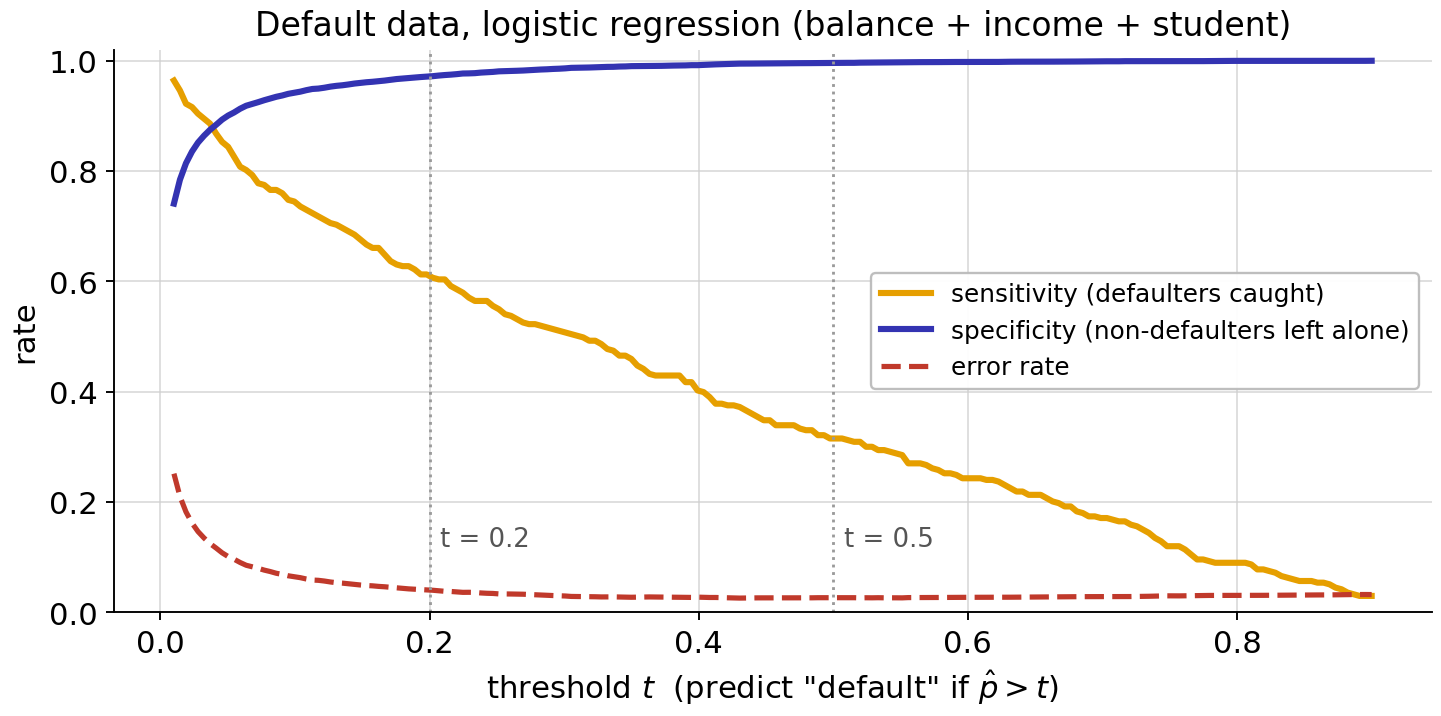
\includegraphics[width=0.9\textwidth,height=0.55\textheight,keepaspectratio]{images/cls_threshold_tradeoff.png}
  \end{center}
  \begin{itemize}\setlength{\itemsep}{2pt}
    \item Lower $t$ $\Rightarrow$ sensitivity $\uparrow$, specificity
          $\downarrow$ -- and vice versa.
    \item The error rate is minimal around $t=0.5$, but that is not
          necessarily the \emph{cheapest} threshold.
  \end{itemize}
\end{frame}

\begin{frame}{The ROC curve}
  \begin{columns}[c]
    \begin{column}{0.5\textwidth}
      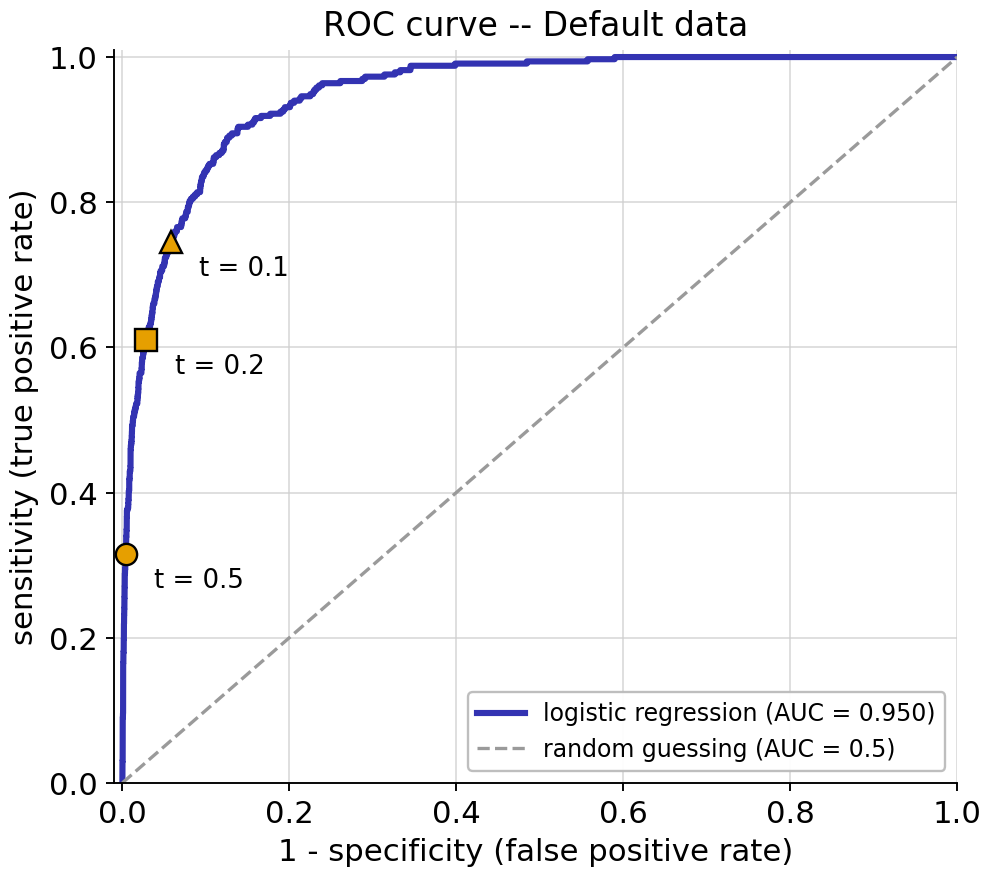
\includegraphics[width=\textwidth,height=0.72\textheight,keepaspectratio]{images/cls_roc.png}
    \end{column}
    \begin{column}{0.48\textwidth}
      \begin{block}{Construction}
        For \emph{every} threshold $t$, plot the pair
        \[
          \bigl(1-\text{specificity},\ \text{sensitivity}\bigr).
        \]
      \end{block}
      \begin{itemize}\setlength{\itemsep}{2pt}
        \item Each point is one threshold; the curve shows all of them.
        \item The diagonal is random guessing.
        \item The closer the curve gets to the \textbf{top-left corner},
              the better the classifier.
      \end{itemize}
    \end{column}
  \end{columns}
\end{frame}

\begin{frame}{AUC -- area under the ROC curve}
  \begin{block}{Definition and interpretation}
    The AUC is the area under the ROC curve. Equivalently,
    \[
      \text{AUC}=P\bigl(\hat p(\text{random defaulter})>\hat p(\text{random non-defaulter})\bigr).
    \]
  \end{block}
  \begin{itemize}\setlength{\itemsep}{3pt}
    \item $\text{AUC}=0.5$: no better than random; $\text{AUC}=1$: perfect
          ranking.
    \item \textbf{Default data:} $\text{AUC}=0.950$ -- a randomly chosen
          defaulter receives a higher predicted probability than a randomly
          chosen non-defaulter in $95\,\%$ of all pairs.
    \item The AUC summarises \textbf{all thresholds} at once -- changing $t$
          moves along the curve but never changes the AUC.
  \end{itemize}
  \kernaussage{The ROC curve and AUC evaluate the \emph{model}; the
  confusion matrix evaluates one \emph{decision rule} (one threshold).}
\end{frame}

\begin{frame}[fragile]{ROC curve and AUC with Python}
  \textbf{Sensitivity and specificity for several thresholds}
  (\texttt{phat} from the model \texttt{g3}):
\begin{lstlisting}
for t in [0.1, 0.2, 0.5]:          # sensitivity, specificity
    print(t, (phat[df.y == 1] > t).mean(), (phat[df.y == 0] <= t).mean())
# 0.1: 0.7447 0.9421   0.2: 0.6096 0.9713   0.5: 0.3153 0.9959
\end{lstlisting}
  \textbf{ROC curve and AUC:}
\begin{lstlisting}
from sklearn.metrics import roc_curve, roc_auc_score
fpr, tpr, thr = roc_curve(df.y, phat)   # one point per threshold
plt.plot(fpr, tpr)                      # ROC curve
plt.plot([0, 1], [0, 1], "--")          # diagonal: random guessing
plt.xlabel("1 - specificity"); plt.ylabel("sensitivity")
print(roc_auc_score(df.y, phat))        # AUC 0.950
\end{lstlisting}
  \inworten{\texttt{phat[df.y == 1]} keeps the defaulters; the mean of
  \texttt{> t} is the share of them that are flagged.}
  \trynotebook{section 5.3 ``ROC curve and AUC''}
\end{frame}

\begin{frame}{Exercise -- threshold, ROC and AUC}
  \begin{block}{Problem statement}
    For the Default model: $t=0.5$ gives sensitivity $0.315$ and
    specificity $0.996$; $t=0.2$ gives sensitivity $0.610$ and specificity
    $0.971$.
    \begin{enumerate}
      \item Locate both operating points on the ROC axes.
      \item How does the point move when the threshold drops from $0.5$ to
            $0.2$?
      \item A colleague hopes to improve the AUC by choosing a better
            threshold. Comment.
    \end{enumerate}
  \end{block}
\end{frame}

\begin{frame}{Solution -- threshold, ROC and AUC}
  \textbf{(1)} $t=0.5$: $(1-0.996,\ 0.315)=(0.004,\ 0.315)$;\\
  \phantom{\textbf{(1)}} $t=0.2$: $(1-0.971,\ 0.610)=(0.029,\ 0.610)$.

  \medskip
  \textbf{(2)} The point moves \textbf{up and to the right along the same
  curve}: a small loss in specificity ($+0.025$ on the $x$-axis) buys a
  large gain in sensitivity ($+0.295$).

  \medskip
  \textbf{(3)} Impossible: the threshold only selects a point \emph{on} the
  curve. The AUC belongs to the model's ranking of the customers -- only a
  better \emph{model} (better variables) can raise it.
  \begin{exampleblock}{Practice}
    Choose the model by its AUC, then choose the threshold by the costs of
    the two error types.
  \end{exampleblock}
\end{frame}

\subsection{Training and test data}

\begin{frame}{Honest evaluation: training and test data}
  \begin{block}{Problem}
    So far we evaluated the model on the \emph{same} data used to fit it.
    This is \textbf{optimistic}: the model has adapted to exactly these
    customers. What counts is the performance on \textbf{new} customers.
  \end{block}
  \begin{block}{Solution: split the data}
    \begin{itemize}
      \item \textbf{Training data} (e.g.\ $70\,\%$): estimate the model.
      \item \textbf{Test data} (the remaining $30\,\%$): compute the
            confusion matrix and the AUC -- data the model has never seen.
    \end{itemize}
  \end{block}
  \begin{exampleblock}{Default data: $7000$ training, $3000$ test customers (\texttt{random\_state=1})}
    At $t=0.5$ the model catches $34$ of $112$ test defaulters, at $t=0.2$
    already $67$. Test AUC $=0.956$ (in-sample on all data: $0.950$) -- with
    only four coefficients there is little to overfit, and chance can even
    push a test value above the in-sample one.
  \end{exampleblock}
\end{frame}

\begin{frame}{Exercise -- training vs.\ test data}
  \begin{block}{Problem statement}
    The model \texttt{default \textasciitilde\ balance + income + student} is
    fitted on $7000$ training customers and applied to the $3000$ test
    customers ($112$ of them defaulted):
    \begin{center}
      \renewcommand{\arraystretch}{1.2}
      \begin{tabular}{lcccc}
        \toprule
        & TN & FP & FN & TP\\
        \midrule
        Test data, $t=0.5$ & $2878$ & $10$ & $78$ & $34$\\
        Test data, $t=0.2$ & $2824$ & $64$ & $45$ & $67$\\
        \bottomrule
      \end{tabular}
    \end{center}
    \begin{enumerate}
      \item Compute accuracy, sensitivity, specificity and precision for
            both thresholds.
      \item On all $10\,000$ customers (training $=$ evaluation data) the
            sensitivity at $t=0.5$ was $0.315$. Compare and explain.
    \end{enumerate}
  \end{block}
\end{frame}

\begin{frame}{Solution -- training vs.\ test data}
  \textbf{(1) Test-data metrics:}
  \begin{center}
    \renewcommand{\arraystretch}{1.2}
    \begin{tabular}{lcc}
      \toprule
      & $t=0.5$ & $t=0.2$\\
      \midrule
      Accuracy & $\frac{2878+34}{3000}=0.971$ & $\frac{2824+67}{3000}=0.964$\\[2pt]
      Sensitivity & $\frac{34}{112}=0.304$ & $\frac{67}{112}=0.598$\\[2pt]
      Specificity & $\frac{2878}{2888}=0.997$ & $\frac{2824}{2888}=0.978$\\[2pt]
      Precision & $\frac{34}{44}=0.773$ & $\frac{67}{131}=0.511$\\
      \bottomrule
    \end{tabular}
  \end{center}
  \textbf{(2)} On new customers the model catches $30.4\,\%$ of the
  defaulters at $t=0.5$, slightly less than the $31.5\,\%$ on the data it was
  fitted on. In-sample figures tend to be \textbf{optimistic}; here the gap is
  small (a simple model, $7000$ training customers), and with only $112$ test
  defaulters part of any difference is chance.

  \medskip
  \inworten{Report the test-data metrics -- they describe what the bank can
  expect for future applicants.}
\end{frame}

\begin{frame}[fragile]{Classification with Python}
  \begin{block}{Predicted probabilities and confusion matrix}
\begin{lstlisting}
phat = g3.predict(df)            # P(default = Yes); log-odds: which="linear"
print(pd.crosstab(df.default, phat > 0.5))     # t = 0.5: 9627 40 / 228 105
\end{lstlisting}
  \end{block}
  \begin{block}{Training and test data, test AUC}
\begin{lstlisting}
from sklearn.metrics import roc_auc_score
train = df.sample(n=7000, random_state=1)      # 70 % training data
test = df.drop(train.index)                    # remaining 30 % test data
g_tr = smf.logit("y ~ balance + income + student", data=train).fit(disp=0)
p_te = g_tr.predict(test)                      # test-set probabilities
print(pd.crosstab(test.default, p_te > 0.5))   # 2878 10 / 78 34
print(roc_auc_score(test.y, p_te))             # test AUC 0.956
\end{lstlisting}
  \end{block}
  \trynotebook{section 5.4 ``Training and test data''}
\end{frame}

% ============================================================================
% SECTION 6: SUMMARY
% ============================================================================
\section{Summary}

\begin{frame}{Summary 1 -- two-way tables and conditional probability}
  \begin{block}{Two-way table of two categorical variables}
    \textbf{joint} relative frequency: cell$/n$; \ \textbf{marginal}: row or
    column total$/n$; \ \textbf{conditional}: cell$/$row (or column) total.
  \end{block}
  \begin{columns}[T]
    \begin{column}{0.49\textwidth}
      \begin{block}{Rules}
        $P(A\mid B)=P(A\cap B)/P(B)$\\[2pt]
        $P(A\cap B)=P(A\mid B)\,P(B)=P(B\mid A)\,P(A)$\\[2pt]
        $P(A\cup B)=P(A)+P(B)-P(A\cap B)$\\[2pt]
        independent: $P(A\cap B)=P(A)\,P(B)\Leftrightarrow P(A\mid B)=P(A)$
      \end{block}
    \end{column}
    \begin{column}{0.49\textwidth}
      \begin{block}{Link to classification}
        Classification estimates $p(x)=P(Y=1\mid X=x)$ -- for a metric $x$
        with a model. Sensitivity $P(\hat y=1\mid y=1)$ and precision
        $P(y=1\mid\hat y=1)$ condition in opposite directions.
      \end{block}
    \end{column}
  \end{columns}
  \inworten{$P(A\mid B)\neq P(B\mid A)$: $4.3\,\%$ of the students
  default, but $38\,\%$ of the defaulters are students.}
\end{frame}

\begin{frame}{Summary 2 -- logistic regression}
  \begin{block}{Model}
    \[
      \log\frac{p(x)}{1-p(x)}=\beta_0+\beta_1x_1+\dots+\beta_px_p,
      \qquad
      p(x)=\frac{e^{\eta}}{1+e^{\eta}}
    \]
    estimated by \textbf{maximum likelihood}.
  \end{block}
  \begin{block}{Interpretation of $\beta_j$ (holding the other variables fixed)}
    \begin{itemize}\setlength{\itemsep}{0pt}
      \item sign: direction of the effect on the probability,
      \item $\beta_j$: change of the log-odds per unit of $x_j$,
      \item $e^{\beta_j}$: \textbf{odds ratio} -- factor by which the odds
            change per unit of $x_j$.
    \end{itemize}
  \end{block}
  \begin{block}{Inference}
    $Z=\hat\beta_j/\mathrm{SE}(\hat\beta_j)\approx N(0,1)$, \
    CI $\hat\beta_j\pm z_{1-\alpha/2}\mathrm{SE}(\hat\beta_j)$, \
    CI for the odds ratio: exponentiate the bounds.
  \end{block}
\end{frame}

\begin{frame}{Summary 3 -- decisions and evaluation}
  \begin{block}{Classification rule}
    $\hat y=1$ if $\hat p(x)>t$ \ $\Leftrightarrow$ \ $\hat\eta(x)>\log\frac{t}{1-t}$;
    \ the threshold $t$ is a business decision.
  \end{block}
  \begin{center}
    \renewcommand{\arraystretch}{1.25}
    \begin{tabular}{l|l|l|l}
      \toprule
      \textbf{Measure} & \textbf{Formula} & \textbf{Probability} & \textbf{Question}\\
      \midrule
      Accuracy & $(\mathrm{TP}+\mathrm{TN})/n$ & $P(\hat y=y)$ & share of correct decisions\\
      Sensitivity & $\mathrm{TP}/(\mathrm{TP}+\mathrm{FN})$ & $P(\hat y=1\mid y=1)$ & share of positives caught\\
      Specificity & $\mathrm{TN}/(\mathrm{TN}+\mathrm{FP})$ & $P(\hat y=0\mid y=0)$ & share of negatives left alone\\
      Precision & $\mathrm{TP}/(\mathrm{TP}+\mathrm{FP})$ & $P(y=1\mid\hat y=1)$ & share of alarms that are real\\
      AUC & area under ROC & -- & ranking over all thresholds\\
      \bottomrule
    \end{tabular}
  \end{center}
  \inworten{precision also depends on the base rate $\pi$:
  $\text{sens}\cdot\pi\,/\,[\text{sens}\cdot\pi+(1-\text{spec})(1-\pi)]$.
  Evaluate on \textbf{test data} the model has not seen.}
\end{frame}

\begin{frame}[fragile]{Summary 4 -- important Python commands}
  \begin{columns}[T]
    \begin{column}{0.5\textwidth}
      \begin{block}{Two-way tables}
\begin{lstlisting}
pd.crosstab(df.a, df.b, margins=True)
pd.crosstab(df.a, df.b,
            normalize="index")  # rows
\end{lstlisting}
      \end{block}
      \begin{block}{Logistic regression}
\begin{lstlisting}
g = smf.logit("y ~ x1 + x2",
              data=df).fit()
print(g.summary())    # z-tests
np.exp(g.params)      # odds ratios
np.exp(g.conf_int())  # CIs for ORs
g.predict(new)        # probabilities
\end{lstlisting}
      \end{block}
    \end{column}
    \begin{column}{0.48\textwidth}
      \begin{block}{Decisions and evaluation}
\begin{lstlisting}
phat = g.predict(df)
pd.crosstab(df.y, phat > 0.5)
pd.crosstab(df.y, phat > 0.5,
            normalize="index")
roc_auc_score(df.y, phat)  # AUC
train = df.sample(n=7000,
                  random_state=1)
test = df.drop(train.index)
\end{lstlisting}
      \end{block}
    \end{column}
  \end{columns}
  \appendixnote{Bayes classifiers in sklearn: \texttt{LinearDiscriminantAnalysis}, \texttt{GaussianNB}}
\end{frame}

\begin{frame}{Six classic pitfalls -- final checklist}
  \small
  \begin{center}
    \renewcommand{\arraystretch}{1.22}
    \begin{tabular}{@{}>{\raggedright\arraybackslash}p{0.43\textwidth}>{\raggedright\arraybackslash}p{0.52\textwidth}@{}}
      \toprule
      \textbf{Forbidden sentence \ \textcolor{hsbirot}{$\times$}} &
      \textbf{Correct version \ \textcolor{hsbigruen}{$\checkmark$}}\\
      \midrule
      ``The odds ratio is $1.78$, so the probability rises by $78\,\%$.'' &
        The \emph{odds} rise by $78\,\%$; the change in probability depends on
        the starting point.\\
      ``Accuracy $97\,\%$ -- an excellent classifier.'' &
        With $3\,\%$ defaulters, always saying ``no'' gives $97\,\%$; check
        sensitivity and specificity.\\
      ``$t=0.5$ is the correct threshold.'' &
        The threshold depends on the costs of the two errors.\\
      ``A better threshold improves the AUC.'' &
        The threshold moves along the ROC curve; only a better model raises
        the AUC.\\
      ``Students are riskier, so reject students.'' &
        At the same balance, students are \emph{less} risky -- ask what is
        held fixed.\\
      ``The test catches $95\,\%$ of the defects, so $95\,\%$ of the
      flagged parts are defective.'' &
        That is $P(+\mid D)$; $P(D\mid +)$ also depends on the base rate --
        with $2\,\%$ defects only $33\,\%$.\\
      \bottomrule
    \end{tabular}
  \end{center}
\end{frame}

\begin{frame}{Looking back: the lecture in one slide}
  \begin{center}
    \small\renewcommand{\arraystretch}{1.22}
    \begin{tabular}{@{}l>{\raggedright\arraybackslash}p{9.6cm}@{}}
      \toprule
      \textbf{Part} & \textbf{Key idea}\\
      \midrule
      1 -- Descriptive Statistics & Summarise data by location and dispersion ($\bar x$, $\tilde x$, $s$, $v$).\\
      2 -- Graphical Representations & Show the distribution: empirical CDF, histogram, boxplot.\\
      3 -- Statistical Inference & Infer from sample to population: estimate $\pm$ critical value $\times$ SE; tests and $p$-values.\\
      4 -- Regression & Explain a metric $Y$ by several $X$ -- with $t$-tests, CIs and diagnostics.\\
      5 -- Classification & Explain a categorical $Y$: logistic regression, decision rules, evaluation.\\
      \bottomrule
    \end{tabular}
  \end{center}
  \kernaussage{One thread through all five parts: every number computed from
  data is an \textbf{estimate} -- describe it, picture it, and report its
  uncertainty.}
\end{frame}


% ============================================================================
% APPENDIX: OPTIONAL AND ADVANCED MATERIAL
% ============================================================================
\appendix
\let\overviewleft\undefined
\section[Appendix]{Appendix: Bayes' Theorem and Generative Classifiers}

\begin{frame}{Appendix -- what is in here, and why}
  \begin{block}{Optional material}
    The main part covers the standard classification workflow with logistic
    regression. The appendix first derives \textbf{Bayes' theorem} -- the
    rule behind the base-rate effect of Section~5 -- and then shows a second
    family of classifiers built on it, useful for small samples, many
    features or more than two classes.
  \end{block}
  \begin{center}
    \small
    \renewcommand{\arraystretch}{1.2}
    \begin{tabular}{@{}l>{\raggedright\arraybackslash}p{9.6cm}@{}}
      \toprule
      \textbf{Topic} & \textbf{Content}\\
      \midrule
      A.1 Bayes' theorem & Total probability, prior $\times$ likelihood $\to$ posterior, taxi example; exercises: suppliers, quality test\\
      A.2 Bayes classifier & Bayes' theorem with classes and features; largest posterior wins\\
      A.3 Naive Bayes & Independent features: the spam filter (exercise)\\
      A.4 LDA & Normal classes with common variance (exercise)\\
      A.5 Comparison & Logistic regression, LDA and naive Bayes; Python commands\\
      \bottomrule
    \end{tabular}
  \end{center}
\end{frame}

\subsection{A.1 Bayes' theorem}

\begin{frame}{Law of total probability}
  \begin{columns}[c]
    \begin{column}{0.47\textwidth}
      \begin{block}{Two cases $B$ and $\bar B$ (``not $B$'')}
        \vspace{-0.5em}
        \[
          P(A)=P(A\mid B)\,P(B)+P(A\mid\bar B)\,P(\bar B)
        \]
        In general, if $B_1,\dots,B_k$ are disjoint and together cover all
        cases: $P(A)=\sum_{j}P(A\mid B_j)\,P(B_j)$.
      \end{block}
    \end{column}
    \begin{column}{0.5\textwidth}
      \centering
      \resizebox{\textwidth}{!}{%
      \begin{tikzpicture}[font=\small,
          every node/.append style={font=\small},
          treelab/.append style={font=\footnotesize}]
        \node[treenode] (r) at (0,0) {all\\cases};
        \node[treenode] (b) at (1.9,1.2) {$B$};
        \node[treenode] (nb) at (1.9,-1.2) {$\bar B$};
        \node[treenodeo,anchor=west] (ba) at (3.9,1.8) {$A$: \ $P(A\mid B)\,P(B)$};
        \node[treenode,anchor=west] (bna) at (3.9,0.65) {$\bar A$};
        \node[treenodeo,anchor=west] (nba) at (3.9,-0.65) {$A$: \ $P(A\mid\bar B)\,P(\bar B)$};
        \node[treenode,anchor=west] (nbna) at (3.9,-1.8) {$\bar A$};
        \draw[treeedge] (r.east) -- node[treelab]{$P(B)$} (b.west);
        \draw[treeedge] (r.east) -- node[treelab]{$P(\bar B)$} (nb.west);
        \draw[treeedge] (b.east) -- node[treelab]{$P(A\mid B)$} (ba.west);
        \draw[treeedge] (b.east) -- (bna.west);
        \draw[treeedge] (nb.east) -- node[treelab]{$P(A\mid\bar B)$} (nba.west);
        \draw[treeedge] (nb.east) -- (nbna.west);
      \end{tikzpicture}}
    \end{column}
  \end{columns}
  \medskip
  \inworten{multiply along each path (multiplication rule) and add up
  \textbf{all paths that end in $A$}.}
  \begin{exampleblock}{Example (Section~5): how often does the rapid test raise an alarm?}
    $P(+)=P(+\mid\text{ill})\,P(\text{ill})+P(+\mid\text{healthy})\,P(\text{healthy})
    =0.9\cdot0.01+0.1\cdot0.99=0.108$
  \end{exampleblock}
\end{frame}

\begin{frame}{Bayes' theorem -- reversing a conditional probability}
  \textbf{Known:} $P(+\mid\text{ill})$. \ \textbf{Wanted:}
  $P(\text{ill}\mid +)$ -- the conditional probability in the other
  direction.\\[3pt]
  \textbf{Step 1:} multiplication rule in both directions,
  $P(A\mid B)\,P(B)=P(A\cap B)=P(B\mid A)\,P(A)$; solve for $P(B\mid A)$.\\
  \textbf{Step 2:} compute the denominator $P(A)$ with the law of total
  probability.
  \begin{block}{Bayes' theorem}
    \vspace{-0.8em}
    \[
      \underbrace{P(B_i\mid A)}_{\text{posterior}}
      =\frac{\overbrace{P(A\mid B_i)}^{\text{likelihood}}\;\overbrace{P(B_i)}^{\text{prior}}}
             {\underbrace{\textstyle\sum_{j}P(A\mid B_j)\,P(B_j)}_{\text{total probability }P(A)}}
      \qquad
      \text{two cases: }\
      P(B\mid A)=\frac{P(A\mid B)\,P(B)}{P(A\mid B)\,P(B)+P(A\mid\bar B)\,P(\bar B)}
    \]
  \end{block}
  \inworten{observe $A$ $\Rightarrow$ update the probabilities of the
  possible explanations $B_i$. Rapid test: $P(\text{ill})=0.01$ $\to$
  $P(\text{ill}\mid +)=0.009/0.108=0.083$.}
\end{frame}

\begin{frame}{Bayes' theorem -- the three building blocks}
  \begin{columns}[T]
    \begin{column}{0.48\textwidth}
      \begin{block}{Prior $P(B_i)$}
        What we know about $B_i$ \emph{before} observing $A$ -- often a known
        share, e.g.\ the base rate of a disease or of defaulters.
      \end{block}
      \begin{block}{Likelihood $P(A\mid B_i)$}
        How probable the observation $A$ is \emph{if} $B_i$ is true -- e.g.\
        the sensitivity of a test.
      \end{block}
      \begin{block}{Posterior $P(B_i\mid A)$}
        What we know about $B_i$ \emph{after} observing $A$ -- the quantity
        we actually want.
      \end{block}
    \end{column}
    \begin{column}{0.48\textwidth}
      \begin{alertblock}{Bayes as a learning rule}
        \[
          P(B_i)\;\xrightarrow{\ \text{observe }A\ }\;P(B_i\mid A)
        \]
        Prior knowledge is updated by data.
      \end{alertblock}
      \begin{exampleblock}{Dictionary for classification}
        \renewcommand{\arraystretch}{1.15}
        \begin{tabular}{@{}ll@{}}
          cases $B_i$ & classes $Y=k$\\
          observation $A$ & features $X=x$\\
          prior $P(B_i)$ & class share $\pi_k$\\
          likelihood & $f_k(x)$ (A.2)\\
        \end{tabular}
      \end{exampleblock}
    \end{column}
  \end{columns}
\end{frame}

\begin{frame}{Worked example: the night-time taxi (1/2)}
  \begin{alertblock}{Scenario}
    At night a taxi causes an accident. A witness says: ``It was a
    \textbf{blue} taxi.'' The town has $5$ blue and $25$ green taxis. Tests
    show that the witness recognises \emph{both} colours correctly in
    $80\,\%$ of the cases. How likely was the taxi really blue?
  \end{alertblock}
  \begin{columns}[c]
    \begin{column}{0.42\textwidth}
      \small
      \textbf{Events:} $B$ $=$ the taxi was really blue, $W$ $=$ the witness
      says ``blue''.\\[3pt]
      \textbf{Prior:} $P(B)=5/30$, \ $P(\bar B)=25/30$.\\[3pt]
      \textbf{Likelihoods:} $P(W\mid B)=0.8$,
      $P(W\mid\bar B)=0.2$ (green mistaken for blue).\\[3pt]
      \textbf{Tree:} natural frequencies -- imagine the scene once with
      each of the $30$ taxis.
    \end{column}
    \begin{column}{0.56\textwidth}
      \centering
      \resizebox{\textwidth}{!}{%
      \begin{tikzpicture}[font=\footnotesize]
        \node[treenode] (r) at (0,0) {$30$ taxis};
        \node[treenode] (b) at (2.6,1.05) {$5$ blue};
        \node[treenode] (g) at (2.6,-1.05) {$25$ green};
        \node[treenodeo,anchor=west] (bw) at (4.8,1.55) {$\mathbf{4}$ say ``blue''};
        \node[treenode,anchor=west] (bg) at (4.8,0.55) {$1$ says ``green''};
        \node[treenodeo,anchor=west] (gw) at (4.8,-0.55) {$\mathbf{5}$ say ``blue''};
        \node[treenode,anchor=west] (gg) at (4.8,-1.55) {$20$ say ``green''};
        \draw[treeedge] (r.east) -- node[treelab]{$5/30$} (b.west);
        \draw[treeedge] (r.east) -- node[treelab]{$25/30$} (g.west);
        \draw[treeedge] (b.east) -- node[treelab]{$0.8$} (bw.west);
        \draw[treeedge] (b.east) -- node[treelab]{$0.2$} (bg.west);
        \draw[treeedge] (g.east) -- node[treelab]{$0.2$} (gw.west);
        \draw[treeedge] (g.east) -- node[treelab]{$0.8$} (gg.west);
      \end{tikzpicture}}
    \end{column}
  \end{columns}
\end{frame}

\begin{frame}{Worked example: the night-time taxi (2/2)}
  \begin{block}{Total probability: when does the witness say ``blue''?}
    \vspace{-0.4em}
    \[
      P(W)=\underbrace{0.8\cdot\tfrac{5}{30}}_{\text{blue, correct}}
      +\underbrace{0.2\cdot\tfrac{25}{30}}_{\text{green, mistaken}}
      =\tfrac{4}{30}+\tfrac{5}{30}=\tfrac{9}{30}=0.3
    \]
  \end{block}
  \begin{columns}[c]
    \begin{column}{0.47\textwidth}
      \begin{block}{Bayes' theorem}
        \vspace{-0.4em}
        \[
          P(B\mid W)=\frac{0.8\cdot\frac{5}{30}}{\frac{9}{30}}
          =\frac{4}{9}=\textbf{0.444}
        \]
      \end{block}
    \end{column}
    \begin{column}{0.51\textwidth}
      \centering\small
      \renewcommand{\arraystretch}{1.25}
      \begin{tabular}{@{}l|cc|c@{}}
        \toprule
        & says ``blue'' & says ``green'' & Total\\
        \midrule
        really blue & $\mathbf{4}$ & $1$ & $5$\\
        really green & $5$ & $20$ & $25$\\
        \midrule
        Total & $\mathbf{9}$ & $21$ & $30$\\
        \bottomrule
      \end{tabular}\\[1pt]
      {\footnotesize counts out of $30$ scenes ($\div30$ = probabilities)}
    \end{column}
  \end{columns}
  \medskip
  \inworten{only $4$ of the $9$ ``blue'' statements are correct -- the other
  $5$ come from the many green taxis. The witness raises the probability from
  $\frac{5}{30}=17\,\%$ (prior) to $44\,\%$ (posterior) -- still less than
  $50\,\%$.}
\end{frame}

\begin{frame}[fragile]{Bayes' theorem with Python}
  \textbf{Night-time taxi} -- one array entry per case $B_i$ (blue, green):
\begin{lstlisting}
prior = np.array([5, 25]) / 30         # P(blue), P(green):         0.1667 0.8333
lik = np.array([0.8, 0.2])             # P(says "blue" | colour)
joint = prior * lik                    # multiplication rule:       0.1333 0.1667
print(joint.sum())                     # total probability P(W):    0.3
print(joint / joint.sum())             # posterior P(colour | W):   0.4444 0.5556
\end{lstlisting}
  \textbf{The same steps as a function} -- rapid test of Section~5:
\begin{lstlisting}
def bayes(prior, lik):
    joint = prior * lik                # prior x likelihood
    return joint / joint.sum()         # divided by the total probability
print(bayes(np.array([0.01, 0.99]), np.array([0.9, 0.1])))   # P(ill | +) 0.0833
\end{lstlisting}
  \inworten{works for any number of cases: put all priors and likelihoods
  into arrays; the posteriors always add up to $1$.}
  \trynotebook{section A.1 ``Bayes' theorem''}
\end{frame}

\begin{frame}{Exercise -- three suppliers}
  \begin{block}{Problem statement}
    An electronics manufacturer buys a component from three suppliers:
    $L_1$ delivers $50\,\%$, $L_2$ $30\,\%$ and $L_3$ $20\,\%$ of the parts.
    Incoming inspection shows that $2\,\%$ of the parts from $L_1$ are
    defective ($D$), $4\,\%$ from $L_2$ and $10\,\%$ from $L_3$. A part is
    taken at random from stock.
    \begin{enumerate}
      \item Write the given numbers as probabilities $P(L_i)$ and
            $P(D\mid L_i)$.
      \item Compute $P(L_i\cap D)$ for $i=1,2,3$.
      \item Compute $P(D)$. How many defective parts are expected among
            $1000$?
      \item Are ``defective'' and ``from $L_1$'' independent?
      \item The part is defective. Compute $P(L_i\mid D)$ for all three
            suppliers. Which supplier is the most likely source?
    \end{enumerate}
  \end{block}
\end{frame}

\begin{frame}{Solution (1/2) -- three suppliers}
  \textbf{(1)} $L_1,L_2,L_3$ split all parts (each part comes from exactly
  one supplier), so the priors add up to $1$. Given: the first two rows of
  the table.

  \medskip
  \textbf{(2)} Multiplication rule $P(L_i\cap D)=P(D\mid L_i)\,P(L_i)$: the
  third row.
  \begin{center}
    \renewcommand{\arraystretch}{1.25}
    \begin{tabular}{@{}lccc@{}}
      \toprule
      & $L_1$ & $L_2$ & $L_3$\\
      \midrule
      prior $P(L_i)$ & $0.5$ & $0.3$ & $0.2$\\
      likelihood $P(D\mid L_i)$ & $0.02$ & $0.04$ & $0.10$\\
      $P(L_i\cap D)$ & $0.02\cdot0.5=\mathbf{0.010}$ & $0.04\cdot0.3=\mathbf{0.012}$ & $0.10\cdot0.2=\mathbf{0.020}$\\
      \bottomrule
    \end{tabular}
  \end{center}
  \inworten{$1\,\%$ of all parts in stock are defective parts from $L_1$,
  $1.2\,\%$ from $L_2$ and $2\,\%$ from $L_3$ -- the \emph{smallest} supplier
  contributes the \emph{most} defective parts.}
\end{frame}

\begin{frame}{Solution (2/2) -- three suppliers}
  \textbf{(3)} Total probability:
  $P(D)=0.010+0.012+0.020=\textbf{0.042}$; among $1000$ parts we expect
  $\textbf{42}$ defective ones ($10$ from $L_1$, $12$ from $L_2$, $20$ from
  $L_3$).

  \medskip
  \textbf{(4)} $P(L_1)\,P(D)=0.5\cdot0.042=0.021\neq0.010=P(L_1\cap D)$
  $\Rightarrow$ \textbf{not independent}; equivalently
  $P(D\mid L_1)=0.02\neq P(D)=0.042$.

  \medskip
  \textbf{(5)} Bayes' theorem $P(L_i\mid D)=P(L_i\cap D)/P(D)$:
  \[
    P(L_1\mid D)=\frac{0.010}{0.042}=\textbf{0.238},\quad
    P(L_2\mid D)=\frac{0.012}{0.042}=\textbf{0.286},\quad
    P(L_3\mid D)=\frac{0.020}{0.042}=\textbf{0.476}
  \]
  The posteriors add up to $1$. The most likely source is $\mathbf{L_3}$
  (largest posterior -- the rule of the Bayes classifier in A.2): although
  $L_3$ delivers only $20\,\%$ of the parts, its high defect rate
  (likelihood) outweighs the small prior.
\end{frame}

\begin{frame}{Exercise -- automated quality test (exam style)}
  \begin{block}{Problem statement}
    In a production line $2\,\%$ of all parts are defective ($D$). An
    automated test raises an alarm ($+$) for a defective part with
    probability $0.95$ and -- wrongly -- for an intact part with probability
    $0.04$.
    \begin{enumerate}
      \item Draw a probability tree and compute $P(D\cap +)$ and
            $P(\bar D\cap +)$.
      \item Compute the probability $P(+)$ that the test raises an alarm.
      \item Compute $P(D\mid +)$. Explain in one sentence why only about a
            third of the flagged parts are defective, although the test
            catches $95\,\%$ of them.
      \item In the language of Section~5: what are the base rate,
            sensitivity, specificity and precision of this test?
    \end{enumerate}
  \end{block}
\end{frame}

\begin{frame}{Solution (1/2) -- automated quality test (exam style)}
  \begin{columns}[c]
    \begin{column}{0.55\textwidth}
      \centering
      \resizebox{\textwidth}{!}{%
      \begin{tikzpicture}[font=\footnotesize]
        \node[treenode] (r) at (0,0) {part};
        \node[treenodeo] (d) at (2.2,1.1) {$D$};
        \node[treenode] (nd) at (2.2,-1.1) {$\bar D$};
        \node[treenodeo,anchor=west] (dp) at (4.0,1.6) {$+$: \ $0.02\cdot0.95=\mathbf{0.0190}$};
        \node[treenode,anchor=west] (dm) at (4.0,0.6) {$-$: \ $0.02\cdot0.05=0.0010$};
        \node[treenodeo,anchor=west] (ndp) at (4.0,-0.6) {$+$: \ $0.98\cdot0.04=\mathbf{0.0392}$};
        \node[treenode,anchor=west] (ndm) at (4.0,-1.6) {$-$: \ $0.98\cdot0.96=0.9408$};
        \draw[treeedge] (r.east) -- node[treelab]{$0.02$} (d.west);
        \draw[treeedge] (r.east) -- node[treelab]{$0.98$} (nd.west);
        \draw[treeedge] (d.east) -- node[treelab]{$0.95$} (dp.west);
        \draw[treeedge] (d.east) -- node[treelab]{$0.05$} (dm.west);
        \draw[treeedge] (nd.east) -- node[treelab]{$0.04$} (ndp.west);
        \draw[treeedge] (nd.east) -- node[treelab]{$0.96$} (ndm.west);
      \end{tikzpicture}}
    \end{column}
    \begin{column}{0.43\textwidth}
      \textbf{(1)} Path rule (multiplication rule):\\[4pt]
      $P(D\cap +)=0.02\cdot0.95=\textbf{0.0190}$,\\[2pt]
      $P(\bar D\cap +)=0.98\cdot0.04=\textbf{0.0392}$.\\[4pt]
      The four path probabilities add up to $1$.
    \end{column}
  \end{columns}
  \medskip
  \textbf{(2)} Total probability -- add both paths that end in ``$+$'':
  \[
    P(+)=P(+\mid D)\,P(D)+P(+\mid\bar D)\,P(\bar D)=0.0190+0.0392=\textbf{0.0582}
  \]
  The larger part of the alarms ($0.0392$ of $0.0582$) comes from
  \emph{intact} parts.
\end{frame}

\begin{frame}{Solution (2/2) -- automated quality test (exam style)}
  \textbf{(3)} Bayes' theorem:
  $\;P(D\mid +)=\dfrac{P(+\mid D)\,P(D)}{P(+)}=\dfrac{0.0190}{0.0582}=\textbf{0.3265}$.
  \begin{columns}[c]
    \begin{column}{0.5\textwidth}
      \small Natural frequencies for $10\,000$ parts:
      \begin{center}
        \renewcommand{\arraystretch}{1.15}
        \begin{tabular}{@{}l|cc|c@{}}
          \toprule
          & no alarm & alarm & Total\\
          \midrule
          intact & $9408$ & $392$ & $9800$\\
          defective & $10$ & $190$ & $200$\\
          \midrule
          Total & $9418$ & $582$ & $10\,000$\\
          \bottomrule
        \end{tabular}
      \end{center}
    \end{column}
    \begin{column}{0.48\textwidth}
      \small Only $190$ of the $582$ alarms are justified:
      $190/582=0.3265$. Because defective parts are rare ($2\,\%$), the
      $4\,\%$ false alarms among the $98\,\%$ intact parts produce more alarms
      than the defective parts themselves.
    \end{column}
  \end{columns}
  \medskip
  \textbf{(4)} Base rate $\pi=0.02$, sensitivity $0.95$, specificity
  $1-0.04=0.96$, precision $\mathbf{0.3265}$ -- the base-rate effect of
  Section~5.
  \begin{alertblock}{Common mistake}
    Confusing $P(D\mid +)$ with $P(+\mid D)$: ``$95\,\%$ of the flagged parts
    are defective'' is wrong.
  \end{alertblock}
\end{frame}

\subsection{A.2 The Bayes classifier}

\begin{frame}{Two ways to obtain $P(Y=k\mid x)$}
  \begin{columns}[T]
    \begin{column}{0.48\textwidth}
      \begin{block}{Discriminative}
        Model $P(Y=1\mid x)$ \textbf{directly}.\\[2pt]
        Example: logistic regression.
      \end{block}
    \end{column}
    \begin{column}{0.48\textwidth}
      \begin{block}{Generative}
        Model how $x$ is distributed \textbf{within each class} and combine
        it with the class frequencies via \textbf{Bayes' theorem}.\\[2pt]
        Examples: naive Bayes, LDA.
      \end{block}
    \end{column}
  \end{columns}
  \medskip
  \begin{exampleblock}{When generative models are useful}
    Small samples, well separated classes, more than two classes -- and
    they make the \textbf{base rate} (prior) explicit, which matters
    whenever one class is rare.
  \end{exampleblock}
\end{frame}

\begin{frame}{Bayes' theorem in the classification setting}
  \begin{block}{Posterior of class $k$ (Bayes' theorem, A.1, with $B_k=\{Y=k\}$, $A=\{X=x\}$)}
    \[
      P(Y=k\mid X=x)=\frac{\pi_k\,f_k(x)}{\sum_{\ell}\pi_\ell\,f_\ell(x)}
    \]
  \end{block}
  \begin{center}
    \renewcommand{\arraystretch}{1.25}
    \begin{tabular}{@{}cl@{}}
      \toprule
      \textbf{Symbol} & \textbf{Meaning}\\
      \midrule
      $\pi_k=P(Y=k)$ & \textbf{prior}: share of class $k$ (e.g.\ $3.33\,\%$ defaulters)\\
      $f_k(x)$ & \textbf{likelihood}: how typical is $x$ for class $k$?\\
      $P(Y=k\mid x)$ & \textbf{posterior}: probability of class $k$ given $x$\\
      \bottomrule
    \end{tabular}
  \end{center}
  \begin{block}{Bayes classifier}
    Assign $x$ to the class with the \textbf{largest posterior} -- for two
    classes: $\hat y=1$ if $P(Y=1\mid x)>0.5$.
  \end{block}
\end{frame}

\begin{frame}{Bayes' theorem as a flow}
  \centering
  \resizebox{\textwidth}{!}{%
  \begin{tikzpicture}[font=\footnotesize,
      op/.style={circle,draw=hsbiblaudunkel,very thick,fill=hsbiblau!8,
                 minimum size=0.75cm,inner sep=0pt,font=\normalsize}]
    \node[flowboxo,text width=2.8cm] (prior) at (0,1.2)
      {\textbf{Prior} $\pi_k$\\[1pt]\scriptsize how frequent is class $k$?};
    \node[flowboxo,text width=2.8cm] (lik) at (0,-1.2)
      {\textbf{Likelihood} $f_k(x)$\\[1pt]\scriptsize how typical is $x$ in class $k$?};
    \node[op] (times) at (3.1,0) {$\times$};
    \node[flowbox,text width=2.0cm] (joint) at (5.5,0) {\textbf{Score}\\ $\pi_k\,f_k(x)$};
    \node[flowboxg,text width=4.2cm] (post) at (10.6,0)
      {\textbf{Posterior}\\[2pt]
       $\displaystyle P(Y=k\mid x)=\frac{\pi_k f_k(x)}{\sum_\ell \pi_\ell f_\ell(x)}$};
    \draw[flowarr] (prior.east) -- (times);
    \draw[flowarr] (lik.east) -- (times);
    \draw[flowarr] (times) -- (joint);
    \draw[flowarr] (joint) -- node[above=1pt,font=\scriptsize,align=center]{divide by\\the sum} (post);
  \end{tikzpicture}}
  \vspace{0.6em}
  \kernaussage{Every generative classifier is this flow -- naive Bayes and LDA
  differ only in \textbf{how they model the likelihood} $f_k(x)$.}
\end{frame}

\subsection{A.3 Naive Bayes}

\begin{frame}{Naive Bayes: an extreme simplification}
  \begin{block}{Assumption}
    Within each class, the explanatory variables are \textbf{independent}:
    \[
      f_k(x)=f_{k1}(x_1)\cdot f_{k2}(x_2)\cdots f_{kp}(x_p).
    \]
  \end{block}
  \begin{itemize}\setlength{\itemsep}{3pt}
    \item Instead of one $p$-dimensional distribution, only $p$
          one-dimensional ones have to be estimated -- e.g.\ simple
          proportions for yes/no features.
    \item The assumption is almost always \emph{wrong} -- yet the
          \emph{ranking} of the cases is often good enough to classify well.
  \end{itemize}
  \inworten{Classic application: spam filters -- each word contributes its
  own factor to the score.}
\end{frame}

\begin{frame}{Exercise -- naive Bayes spam filter}
  \begin{block}{Problem statement}
    A spam filter has priors $P(\text{Spam})=0.4$, $P(\text{Ham})=0.6$ and two
    binary features: $F_1$ (``contains the word \emph{free}'') and $F_2$
    (``contains a link'').
    \begin{center}
      \renewcommand{\arraystretch}{1.2}
      \begin{tabular}{lcc}
        \toprule
        & $P(F_1=1\mid\cdot)$ & $P(F_2=1\mid\cdot)$\\
        \midrule
        Spam & $0.6$ & $0.7$\\
        Ham & $0.1$ & $0.2$\\
        \bottomrule
      \end{tabular}
    \end{center}
    A new e-mail contains \emph{both} features.
    \begin{enumerate}
      \item Compute the score $\pi_k\,f_k(x)$ of each class.
      \item Compute $P(\text{Spam}\mid F_1=1,F_2=1)$ and classify the e-mail.
    \end{enumerate}
  \end{block}
\end{frame}

\begin{frame}{Solution -- naive Bayes spam filter}
  \begin{exampleblock}{(1) Scores (prior $\times$ product of the feature probabilities)}
    \[
      \text{Spam: } 0.4\cdot0.6\cdot0.7=0.168,
      \qquad
      \text{Ham: } 0.6\cdot0.1\cdot0.2=0.012
    \]
  \end{exampleblock}
  \begin{exampleblock}{(2) Posterior}
    \[
      P(\text{Spam}\mid F_1,F_2)=\frac{0.168}{0.168+0.012}=\frac{0.168}{0.180}=\textbf{0.933}
      \;>\;0.5\;\Rightarrow\;\textbf{Spam}
    \]
  \end{exampleblock}
  \inworten{The two features together are $21$ times as likely under Spam as
  under Ham ($0.42/0.02$); this overwhelms the prior, which favoured Ham.}
  \begin{alertblock}{Common mistake}
    Ignoring the prior: $0.42/(0.42+0.02)=0.955$ overstates the spam
    probability. With rare positives the prior can even flip the decision.
  \end{alertblock}
\end{frame}

\subsection{A.4 Linear discriminant analysis}

\begin{frame}{Linear discriminant analysis (LDA) with one variable}
  \begin{block}{Assumption}
    Within each class, $X$ is \textbf{normally distributed} with mean $\mu_k$
    and a \textbf{common} variance $\sigma^2$: $\;X\mid Y=k\sim N(\mu_k,\sigma^2)$.
  \end{block}
  \begin{block}{Discriminant score and decision boundary (two classes)}
    Inserting the normal densities into Bayes' theorem and taking logs gives
    a score \textbf{linear} in $x$:
    \[
      \delta_k(x)=x\,\frac{\mu_k}{\sigma^2}-\frac{\mu_k^2}{2\sigma^2}+\log\pi_k,
      \qquad
      x^\star=\frac{\mu_0+\mu_1}{2}-\frac{\sigma^2}{\mu_1-\mu_0}\,\log\frac{\pi_1}{\pi_0}.
    \]
    Assign the class with the larger score; at $x^\star$ both scores are equal.
  \end{block}
  \inworten{Equal priors: the boundary is the midpoint of the means. A rare
  class~1 pushes the boundary towards $\mu_1$.}
\end{frame}

\begin{frame}{LDA with one variable -- in pictures}
  \begin{center}
    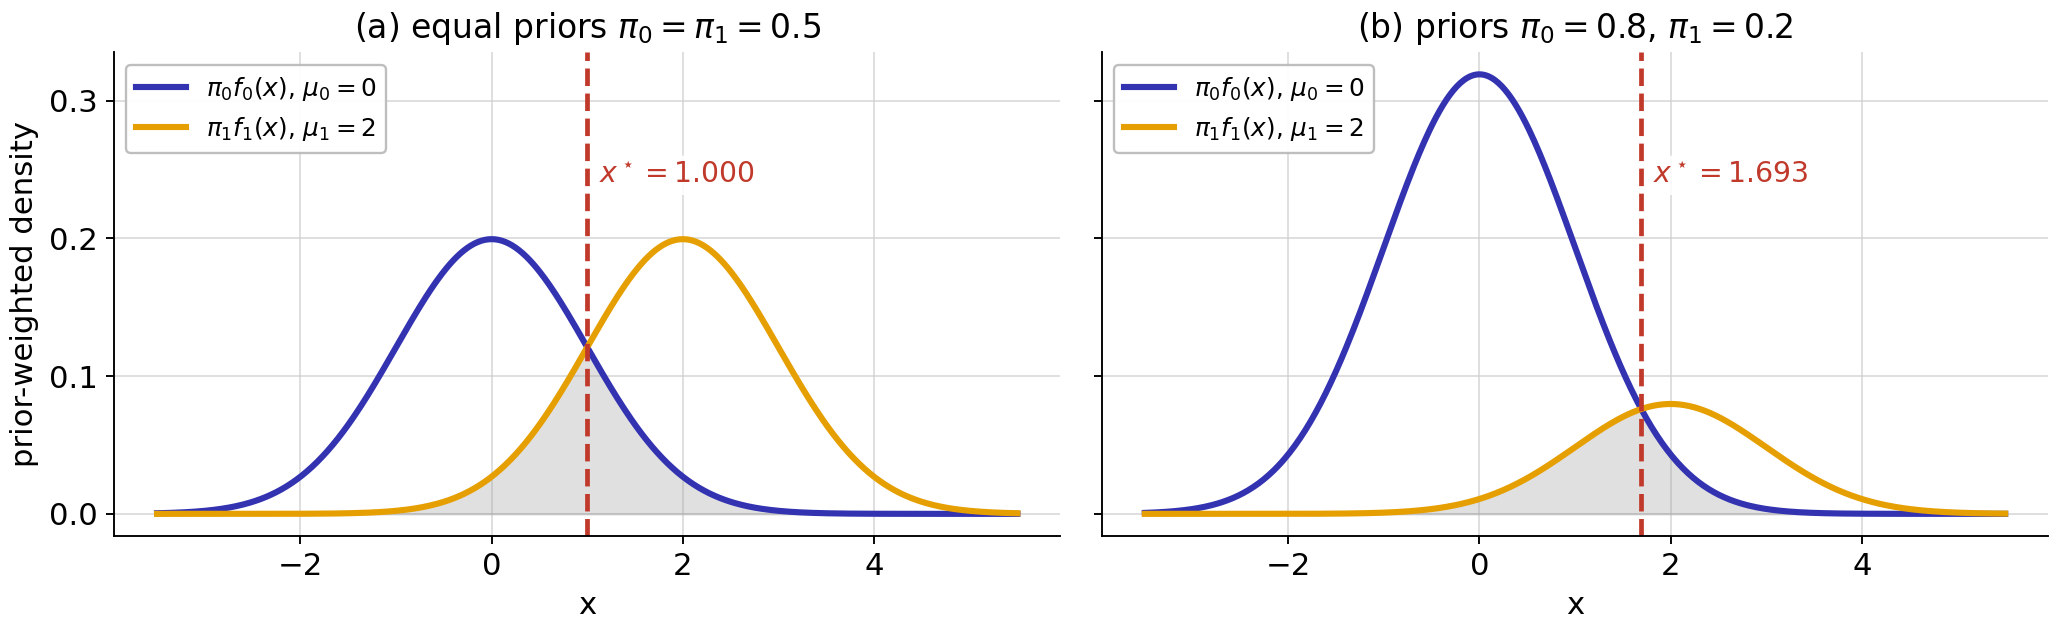
\includegraphics[width=0.95\textwidth,height=0.52\textheight,keepaspectratio]{images/cls_lda_1d.png}
  \end{center}
  \begin{itemize}\setlength{\itemsep}{2pt}
    \item LDA compares the \textbf{prior-weighted densities}
          $\pi_kf_k(x)$; the boundary lies where they cross.
    \item The grey overlap is the error that \emph{no} classifier can avoid.
  \end{itemize}
\end{frame}

\begin{frame}{Exercise -- LDA in one dimension}
  \begin{block}{Problem statement}
    Two classes with $X\mid Y=k\sim N(\mu_k,\sigma^2)$, $\sigma^2=1$,
    $\mu_0=0$, $\mu_1=2$.
    \begin{enumerate}
      \item With equal priors, write down $\delta_0(x)$ and $\delta_1(x)$
            and find the decision boundary.
      \item Classify $x=1.5$.
      \item Now take $\pi_0=0.8$, $\pi_1=0.2$. Recompute the boundary and
            reclassify $x=1.5$.
    \end{enumerate}
  \end{block}
\end{frame}

\begin{frame}{Solution -- LDA in one dimension}
  \begin{exampleblock}{(1)--(2) Equal priors}
    $\delta_0(x)=0+\log0.5$, \quad $\delta_1(x)=2x-2+\log0.5$. The equal
    $\log\pi_k$ terms cancel: $0=2x-2$ $\Rightarrow$ $x^\star=1$ (the midpoint
    of the means). $x=1.5>1$ $\Rightarrow$ \textbf{class 1}.
  \end{exampleblock}
  \begin{exampleblock}{(3) Unequal priors}
    $\delta_0=\log0.8=-0.223$, \quad $\delta_1=2x-2+\log0.2=2x-3.609$:
    \[
      -0.223=2x-3.609\;\Rightarrow\;x^\star=1.693
      \qquad\Bigl(\text{check: }1-\tfrac12\log\tfrac{0.2}{0.8}=1+0.693\ \checkmark\Bigr)
    \]
    Now $x=1.5<1.693$ $\Rightarrow$ \textbf{class 0}.
  \end{exampleblock}
  \inworten{Same observation, opposite decision -- purely because class 1
  became rare: the rarer class needs stronger evidence.}
\end{frame}

\subsection{A.5 Comparison}

\begin{frame}{Logistic regression, LDA and naive Bayes}
  \begin{center}
    \small
    \renewcommand{\arraystretch}{1.22}
    \begin{tabular}{@{}>{\raggedright\arraybackslash}p{2.6cm}*{3}{>{\raggedright\arraybackslash}p{3.5cm}}@{}}
      \toprule
      & \textbf{Logistic regression} & \textbf{LDA} & \textbf{Naive Bayes}\\
      \midrule
      Models & $P(Y=1\mid x)$ directly & normal $f_k$, common variance & independent features\\
      Boundary & linear in $x$ & linear in $x$ & flexible\\
      Strength & few assumptions; interpretable odds ratios, tests & stable for small $n$, several classes & very many features, small $n$\\
      Weakness & unstable if classes are perfectly separated & wrong if normality fails & miscalibrated probabilities\\
      \bottomrule
    \end{tabular}
  \end{center}
  \begin{exampleblock}{Default data (all customers, $t=0.5$)}
    LDA (\texttt{balance + student}) catches $81$ of $333$ defaulters with
    $23$ false alarms; logistic regression catches $105$ with $40$ false
    alarms -- similar trade-offs, AUC around $0.95$ for both.
  \end{exampleblock}
\end{frame}

\begin{frame}[fragile]{Bayes classifiers with Python}
  \begin{block}{Linear discriminant analysis}
\begin{lstlisting}
from sklearn.discriminant_analysis import LinearDiscriminantAnalysis
X = pd.get_dummies(df[["balance", "student"]], drop_first=True)
lda = LinearDiscriminantAnalysis().fit(X, df.default)
print(pd.crosstab(df.default, lda.predict(X)))   # 9644 23 / 252 81
\end{lstlisting}
  \end{block}
  \begin{block}{Naive Bayes}
\begin{lstlisting}
from sklearn.naive_bayes import GaussianNB
nb = GaussianNB().fit(X, df.default)       # normal f_kj for every feature
print(pd.crosstab(df.default, nb.predict(X)))
\end{lstlisting}
  \end{block}
  \trynotebook{section A.5 ``Comparison''}
\end{frame}

\begin{frame}{Appendix summary -- Bayes' theorem and Bayes classifiers}
  \begin{block}{Total probability and Bayes' theorem}
    \vspace{-0.4em}
    \[
      P(A)=\sum_jP(A\mid B_j)\,P(B_j),
      \qquad
      P(B_i\mid A)=\frac{P(A\mid B_i)\,P(B_i)}{P(A)}
    \]
    \inworten{posterior $\propto$ likelihood $\times$ prior; the
    denominator comes from the law of total probability.}\\[2pt]
    Classes and features: \
    $P(Y=k\mid x)=\pi_k\,f_k(x)\big/\sum_\ell\pi_\ell\,f_\ell(x)$; the Bayes
    classifier picks the largest posterior.
  \end{block}
  \begin{itemize}\setlength{\itemsep}{3pt}
    \item \textbf{Naive Bayes:} $f_k(x)=\prod_jf_{kj}(x_j)$ -- independent
          features within each class.
    \item \textbf{LDA:} normal $f_k$ with common variance; one variable:
          boundary
          $x^\star=\frac{\mu_0+\mu_1}{2}-\frac{\sigma^2}{\mu_1-\mu_0}\log\frac{\pi_1}{\pi_0}$.
    \item A rare class needs stronger evidence -- the prior shifts the
          boundary.
  \end{itemize}
\end{frame}

\end{document}
